\subsection{Single Object Visualization}

\subsubsection{Object A}
In this section, 87 pictures of Kobe, filmed from different viewpoints, are trained. It takes about \textbf{2min} to extract pose with COLMAP and \textbf{52:11min}(20000 epochs) to train.

One of the original pictures and the rendering results are as follow(the training dynamics will be posed later with the background scene):


\begin{figure}[H]
	\centering
	

	\begin{subfigure}{0.25\textwidth}
		\centering
		\includegraphics[width=\linewidth]{figures/task1/objectA/Kobe_mesh.png}
		\caption{Kobe Mesh(Floating points and background are manually eliminated)}
	\end{subfigure}
	\hfill
	\begin{subfigure}{0.25\textwidth}
		\centering
		\includegraphics[width=\linewidth]{figures/task1/objectA/Kobe_color.png}
		\caption{Kobe Color}
	\end{subfigure}
	\hfill
	\begin{subfigure}{0.25\textwidth}
		\centering
		\includegraphics[width=\linewidth]{figures/task1/objectA/original_Kobe.jpg}
		\caption{Original Kobe}
	\end{subfigure}
\end{figure}

We can see that the reconstruction has a relatively good fit, the detailed quality analysis will be shown later in Figure~\ref{fig:2DGS Dynamics}

\subsubsection{Object B}
In this section, 2 examples are trained, the prompt are as follow:
\begin{itemize}
	\item A zoomed-out DSLR photo of a baby bunny sitting on top of a stack of pancakes.
	\item A Michelangelo-style statue of an astronaut.
\end{itemize}

Each training takes about \textbf{20 minutes}(10000 epochs), the rendering results and training dynamics are as follow:

\begin{figure}[H]
	\centering
	
	%================ 第一组：Astronaut =================
	\begin{subfigure}{0.25\textwidth}
		\centering
		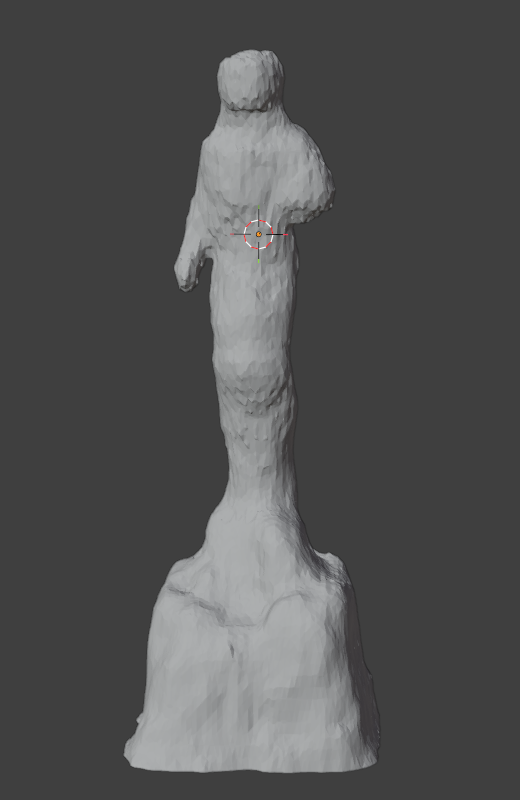
\includegraphics[width=\linewidth]{figures/task1/objectB/astronaut_mesh.png}
		\caption{Astronaut Mesh}
	\end{subfigure}
	\hfill
	\begin{subfigure}{0.25\textwidth}
		\centering
		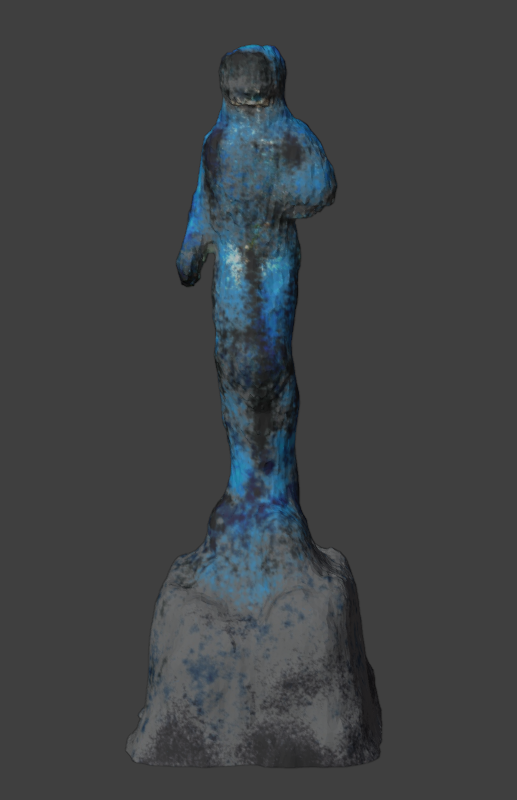
\includegraphics[width=\linewidth]{figures/task1/objectB/astronaut_color.png}
		\caption{Astronaut Color}
		\label{Astronaut Color}
	\end{subfigure}
	\hfill
	\begin{subfigure}{0.25\textwidth}
		\centering
		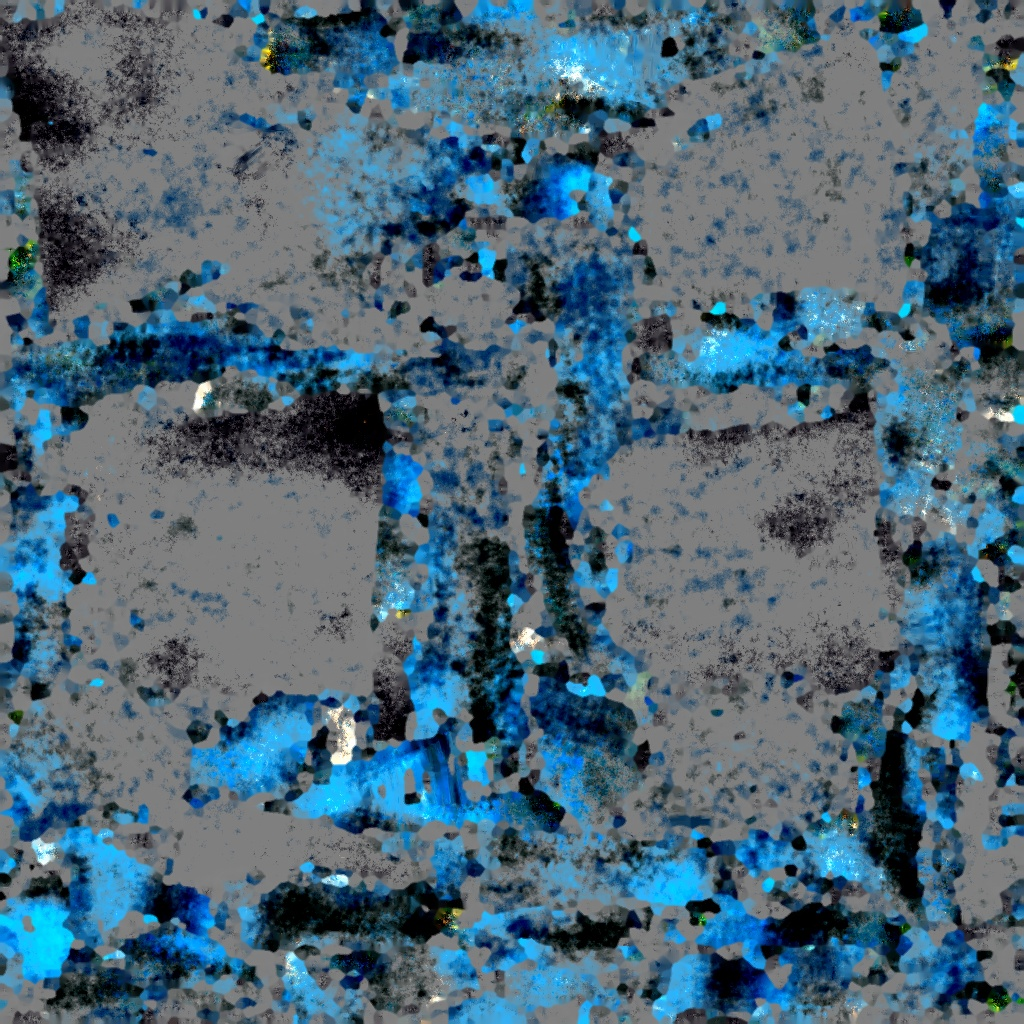
\includegraphics[width=\linewidth]{figures/task1/objectB/astronaut_texture_kd.jpg}
		\caption{Astronaut Texture}
	\end{subfigure}
	
	\vspace{0.6cm}
	
	%================ 第二组：Bunny =================
		% 第一张图（左边）
	\begin{subfigure}{0.8\textwidth}
		\centering
		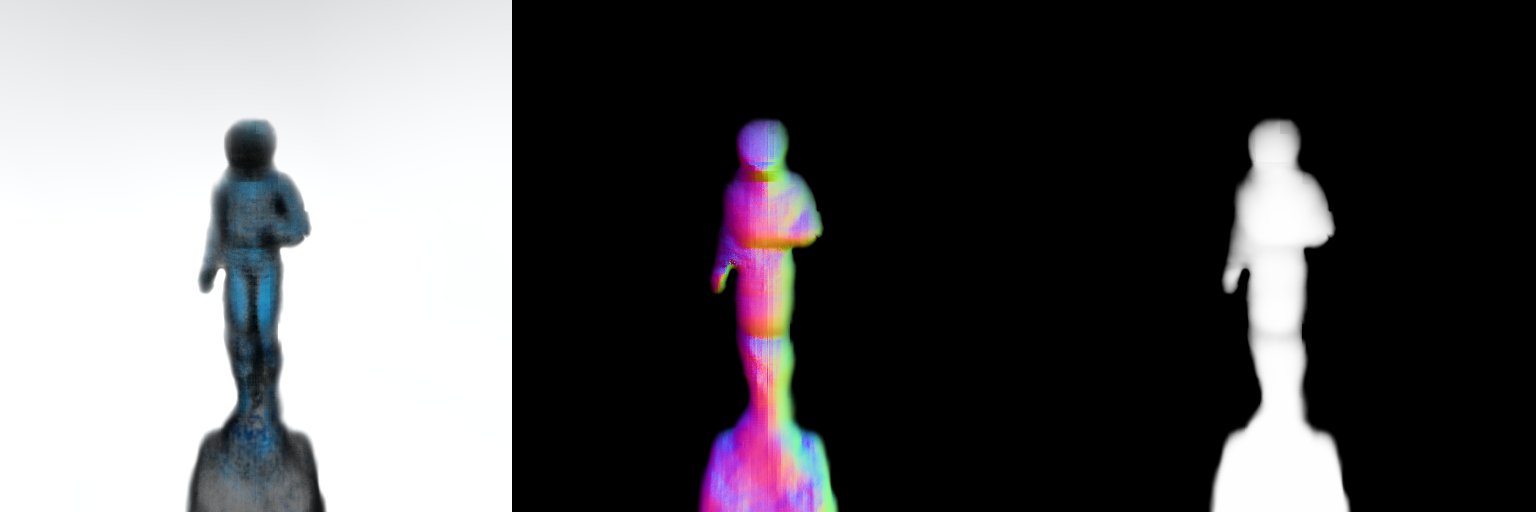
\includegraphics[width=\linewidth]{figures/task1/objectB/astronauts.png} % 替换为你的第一张图片路径
		\caption{Astronauts} % 替换为你想要的图注
	\end{subfigure}
	\hfill % 左右两张图之间的弹性间距

\end{figure}



\begin{figure}[H]
		\begin{subfigure}{0.25\textwidth}
		\centering
		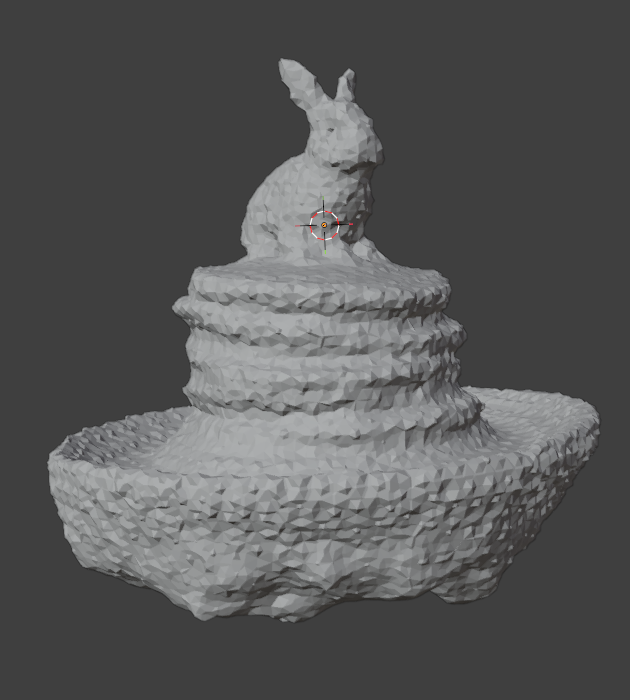
\includegraphics[width=\linewidth]{figures/task1/objectB/bunny_mesh.png}
		\caption{Bunny Mesh}
	\end{subfigure}
	\hfill
	\begin{subfigure}{0.25\textwidth}
		\centering
		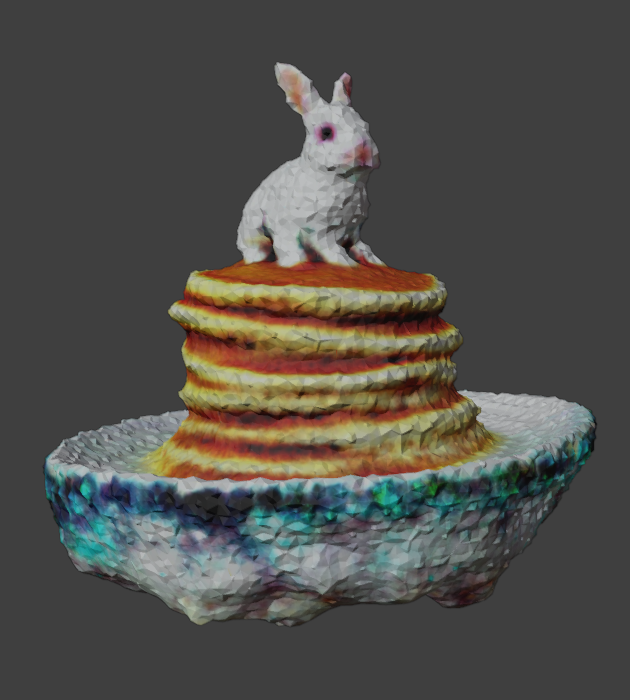
\includegraphics[width=\linewidth]{figures/task1/objectB/bunny_color.png}
		\caption{Bunny Color}
	\end{subfigure}
	\hfill
	\begin{subfigure}{0.25\textwidth}
		\centering
		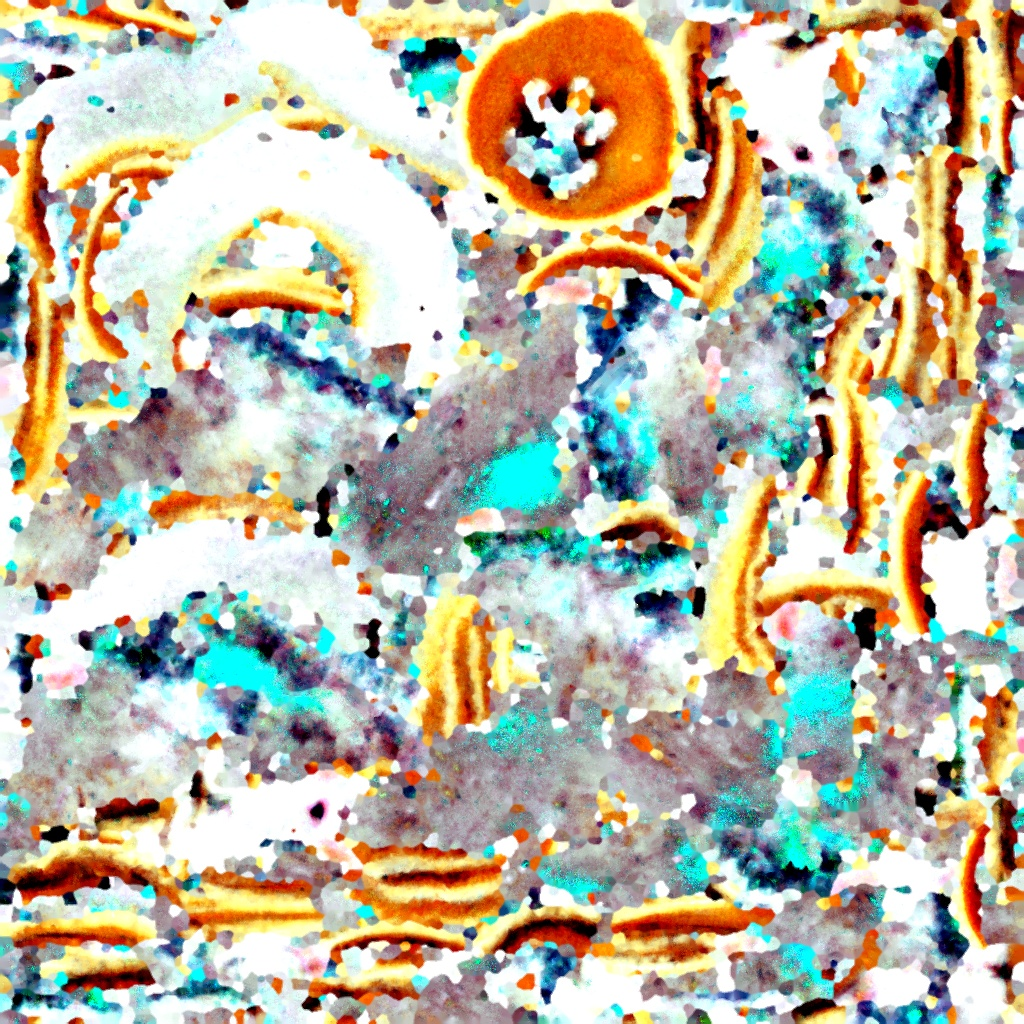
\includegraphics[width=\linewidth]{figures/task1/objectB/bunny_texture_kd.jpg}
		\caption{Bunny Texture}
	\end{subfigure}
	
	\centering
	\vspace{0.6cm}

	% 第二张图（右边）
	\begin{subfigure}{0.8\textwidth}
		\centering
		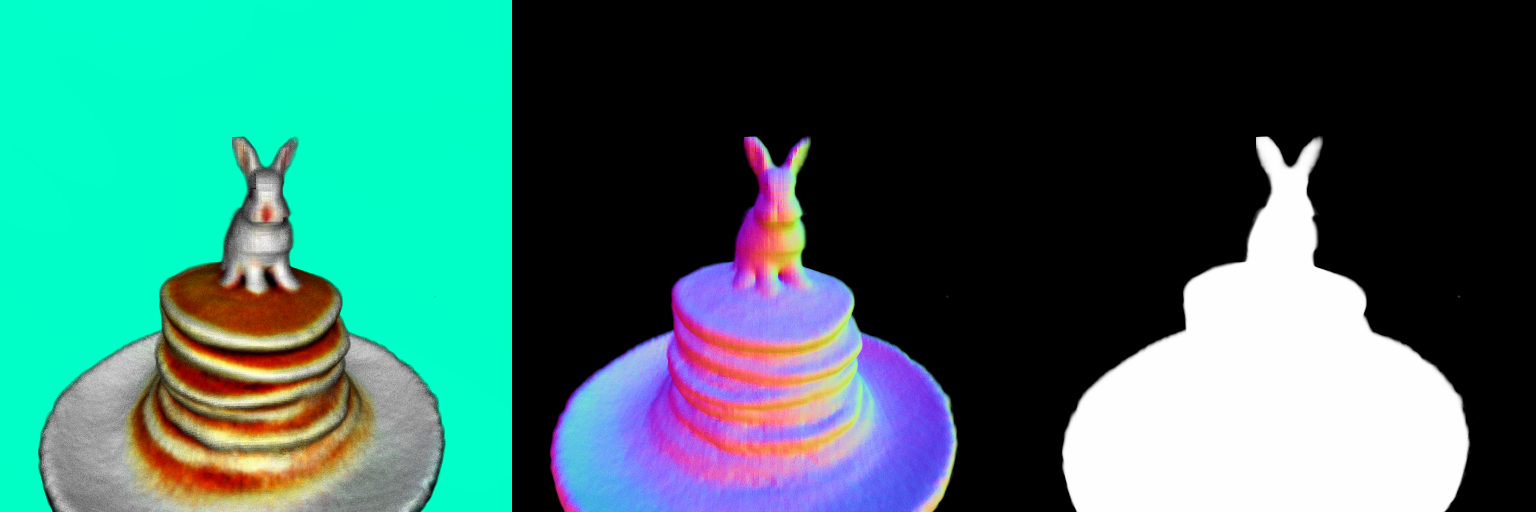
\includegraphics[width=\linewidth]{figures/task1/objectB/bunnys.png} % 替换为你的第二张图片路径
		\caption{Bunnys} % 替换为你想要的图注
	\end{subfigure}

\end{figure}


%================ Loss Functions =================
\begin{figure}[H]
	\centering
	
	% 第一行
	\begin{subfigure}{0.4\textwidth}
		\centering
		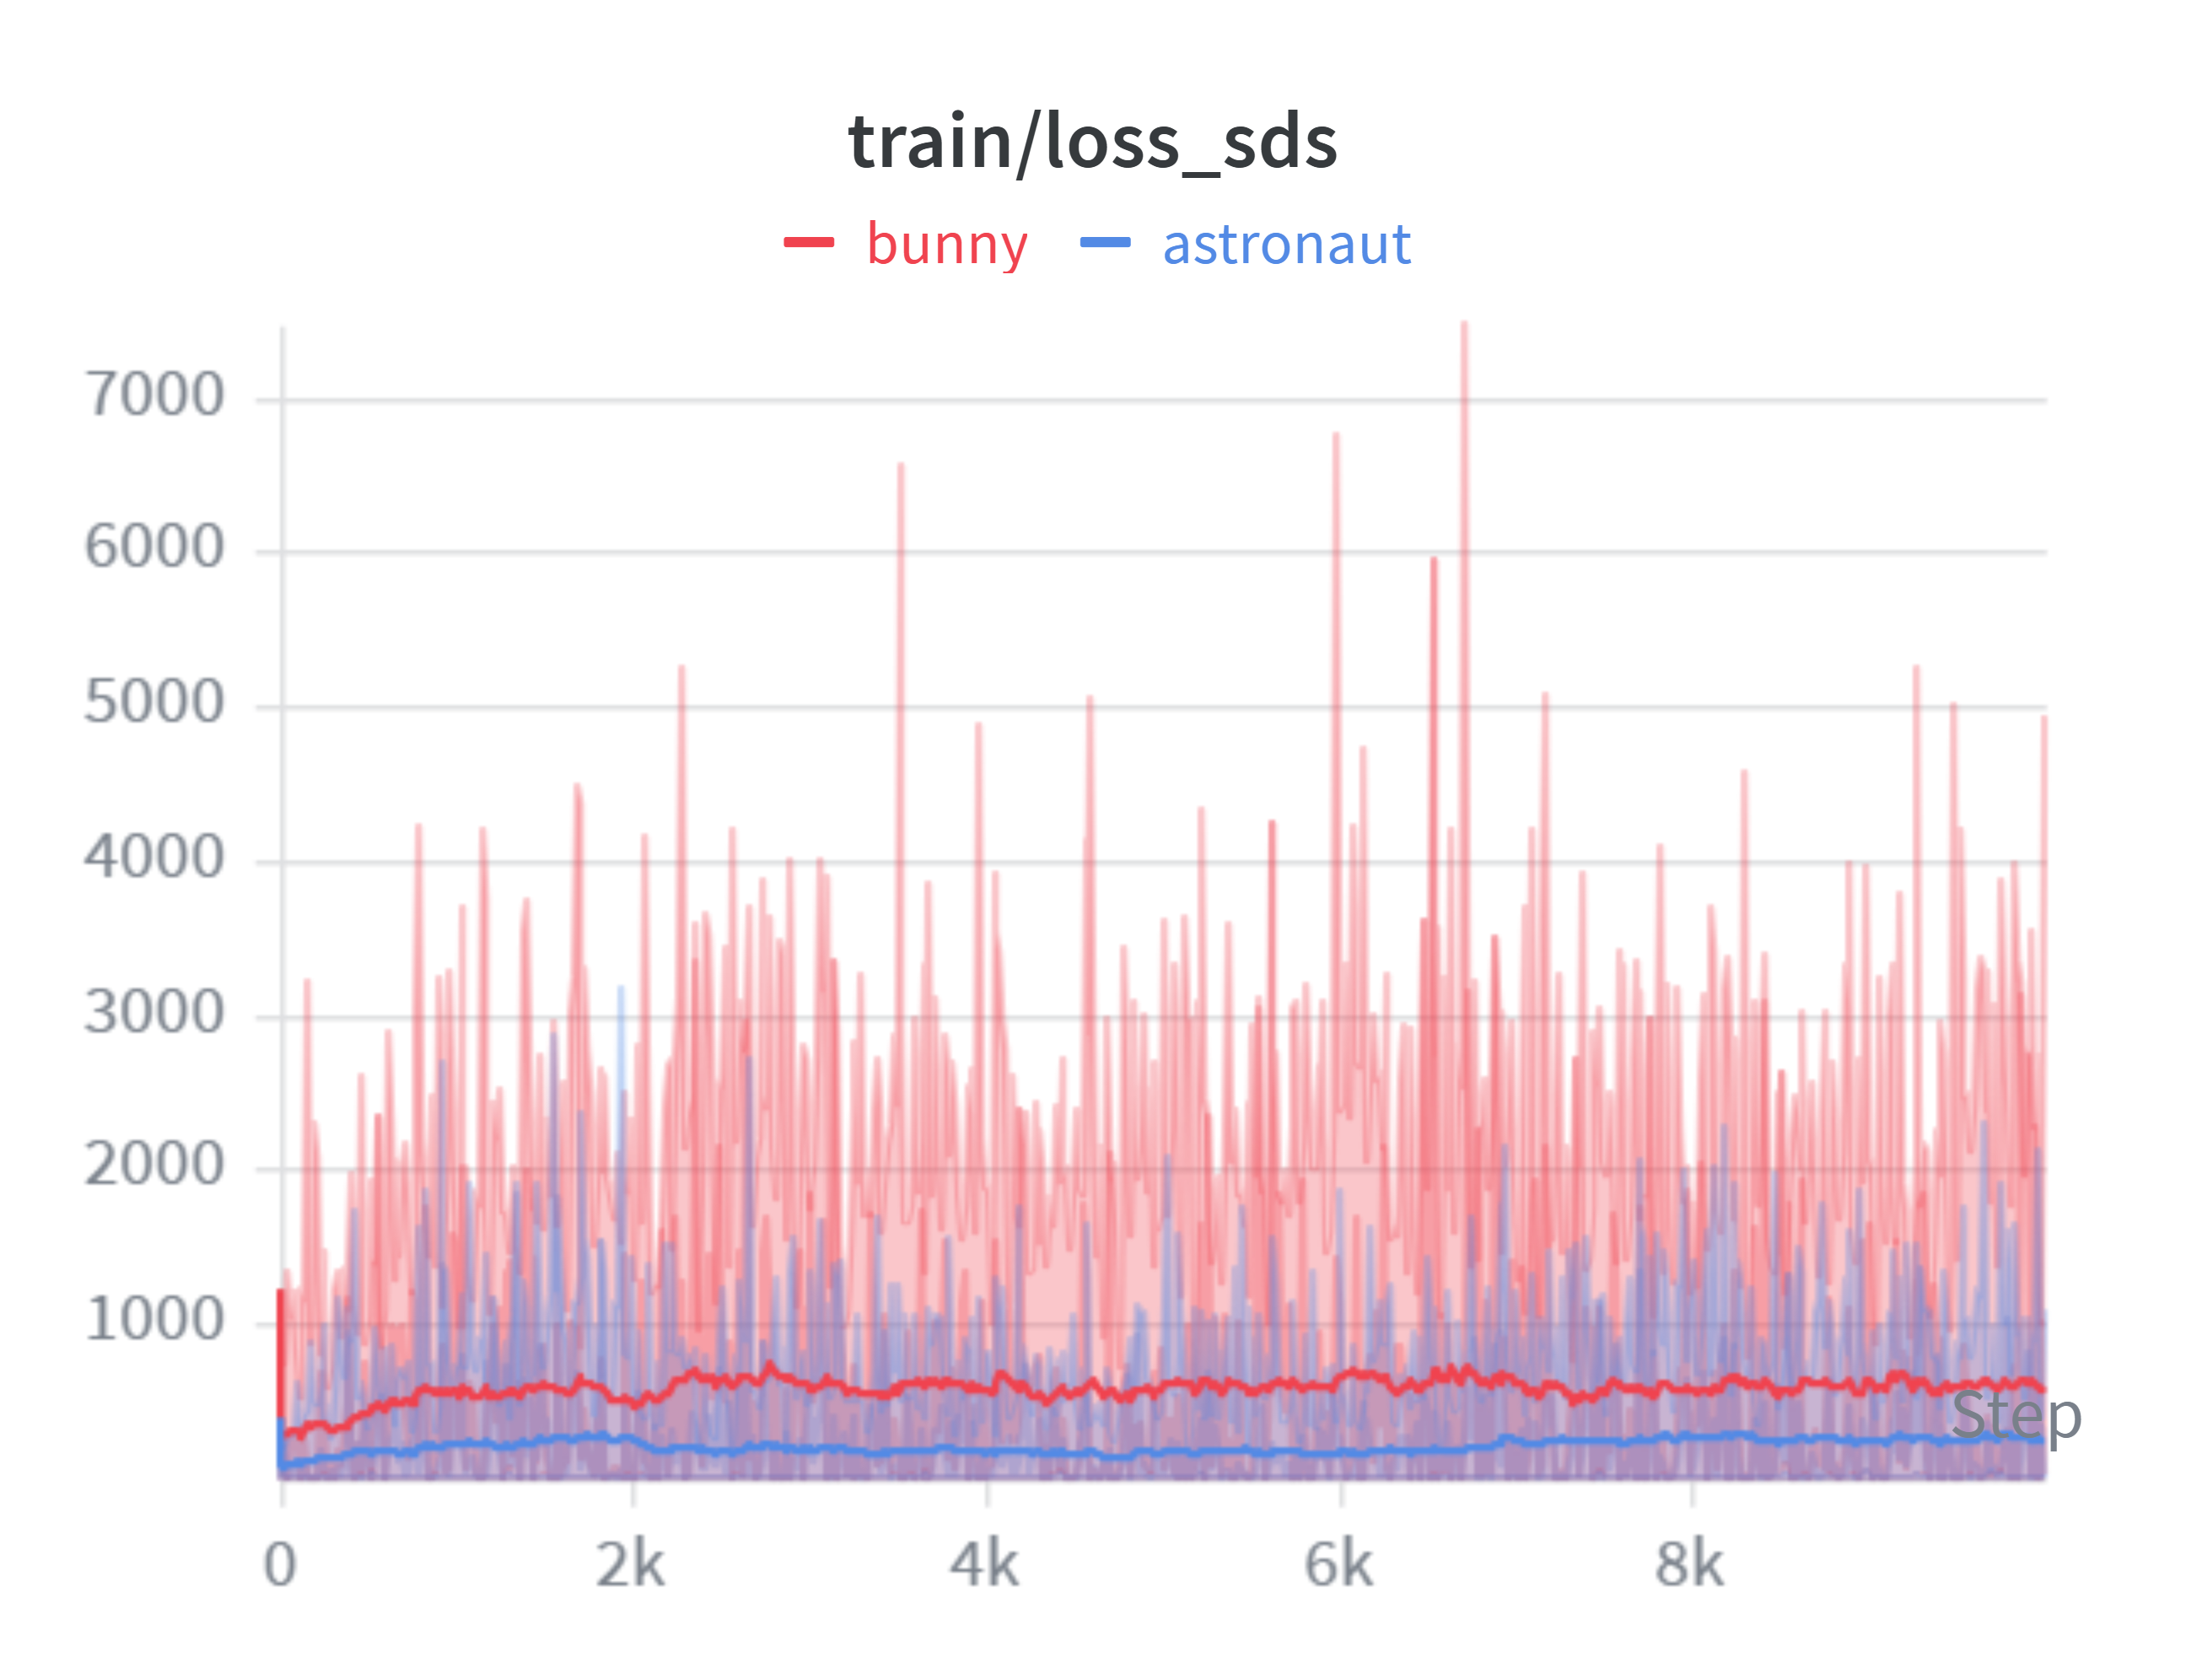
\includegraphics[width=\linewidth]{figures/task1/objectB/sds_loss.png}
		\caption{SDS Loss}
	\end{subfigure}
	\hfill
	\begin{subfigure}{0.4\textwidth}
		\centering
		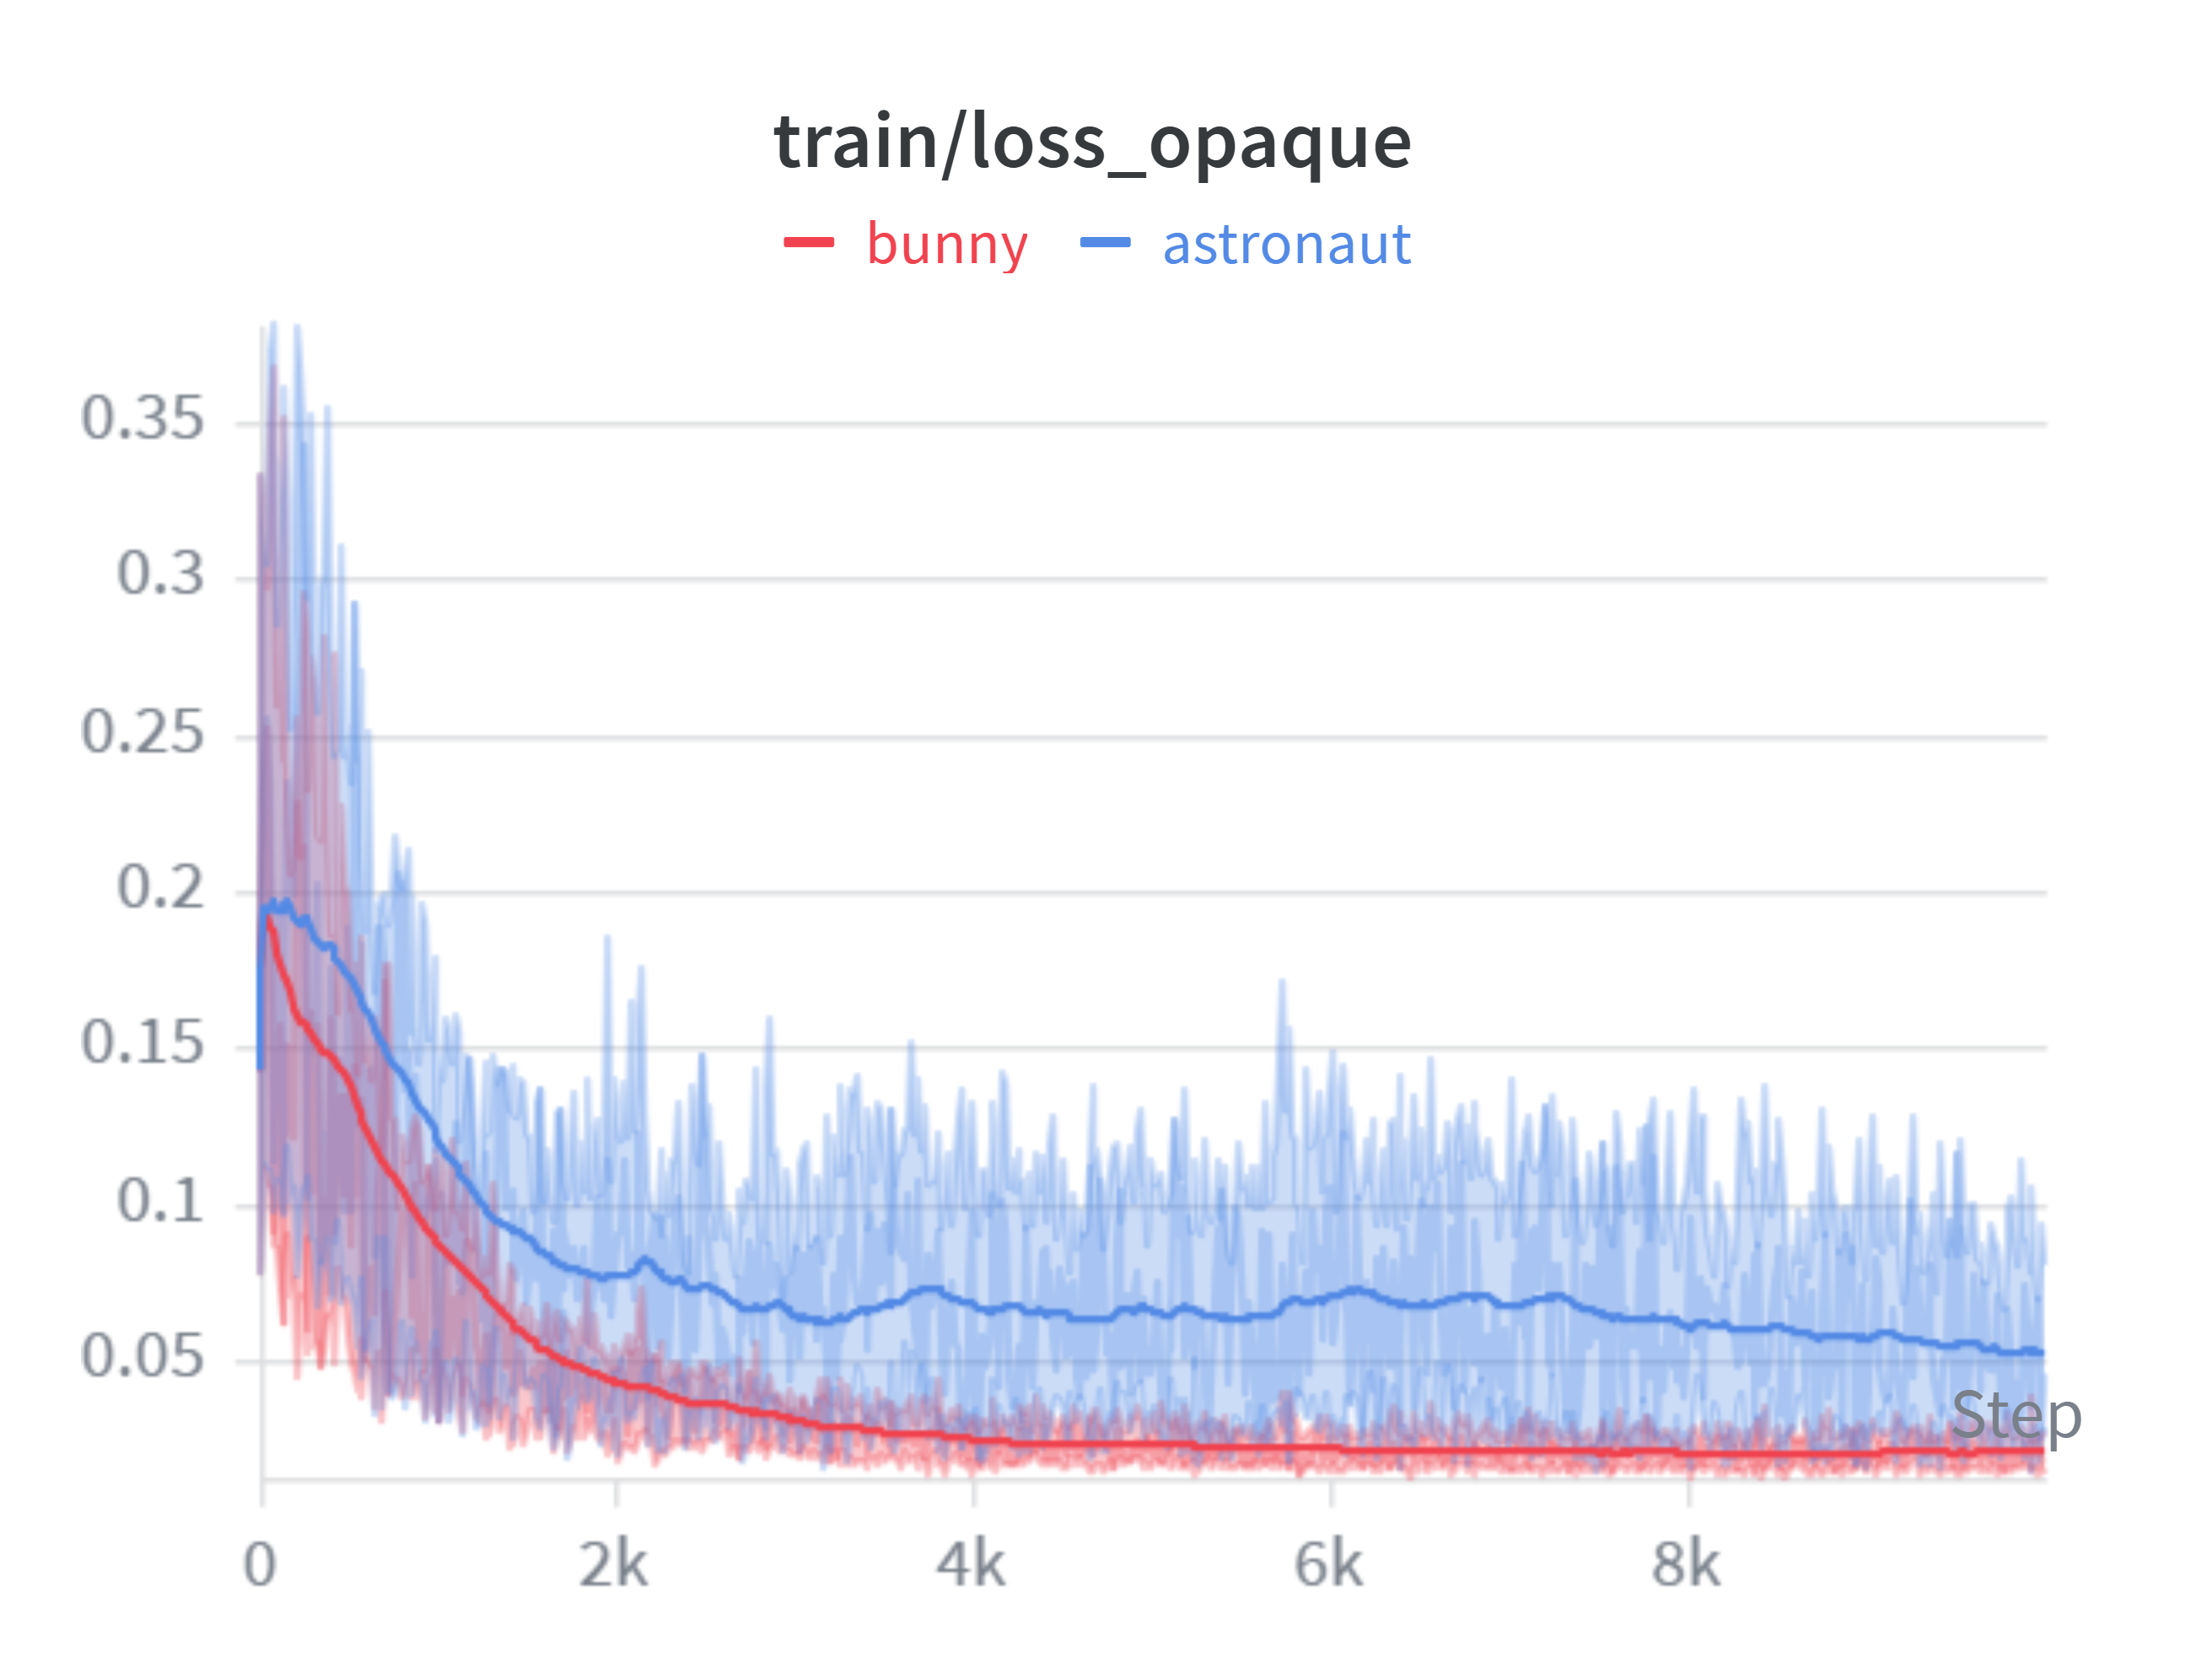
\includegraphics[width=\linewidth]{figures/task1/objectB/opaque_loss.png}
		\caption{Opaque Loss}
	\end{subfigure}
	
	\vspace{0.5cm} % 行间距，可以根据需要调整
	
	% 第二行
	\begin{subfigure}{0.4\textwidth}
		\centering
		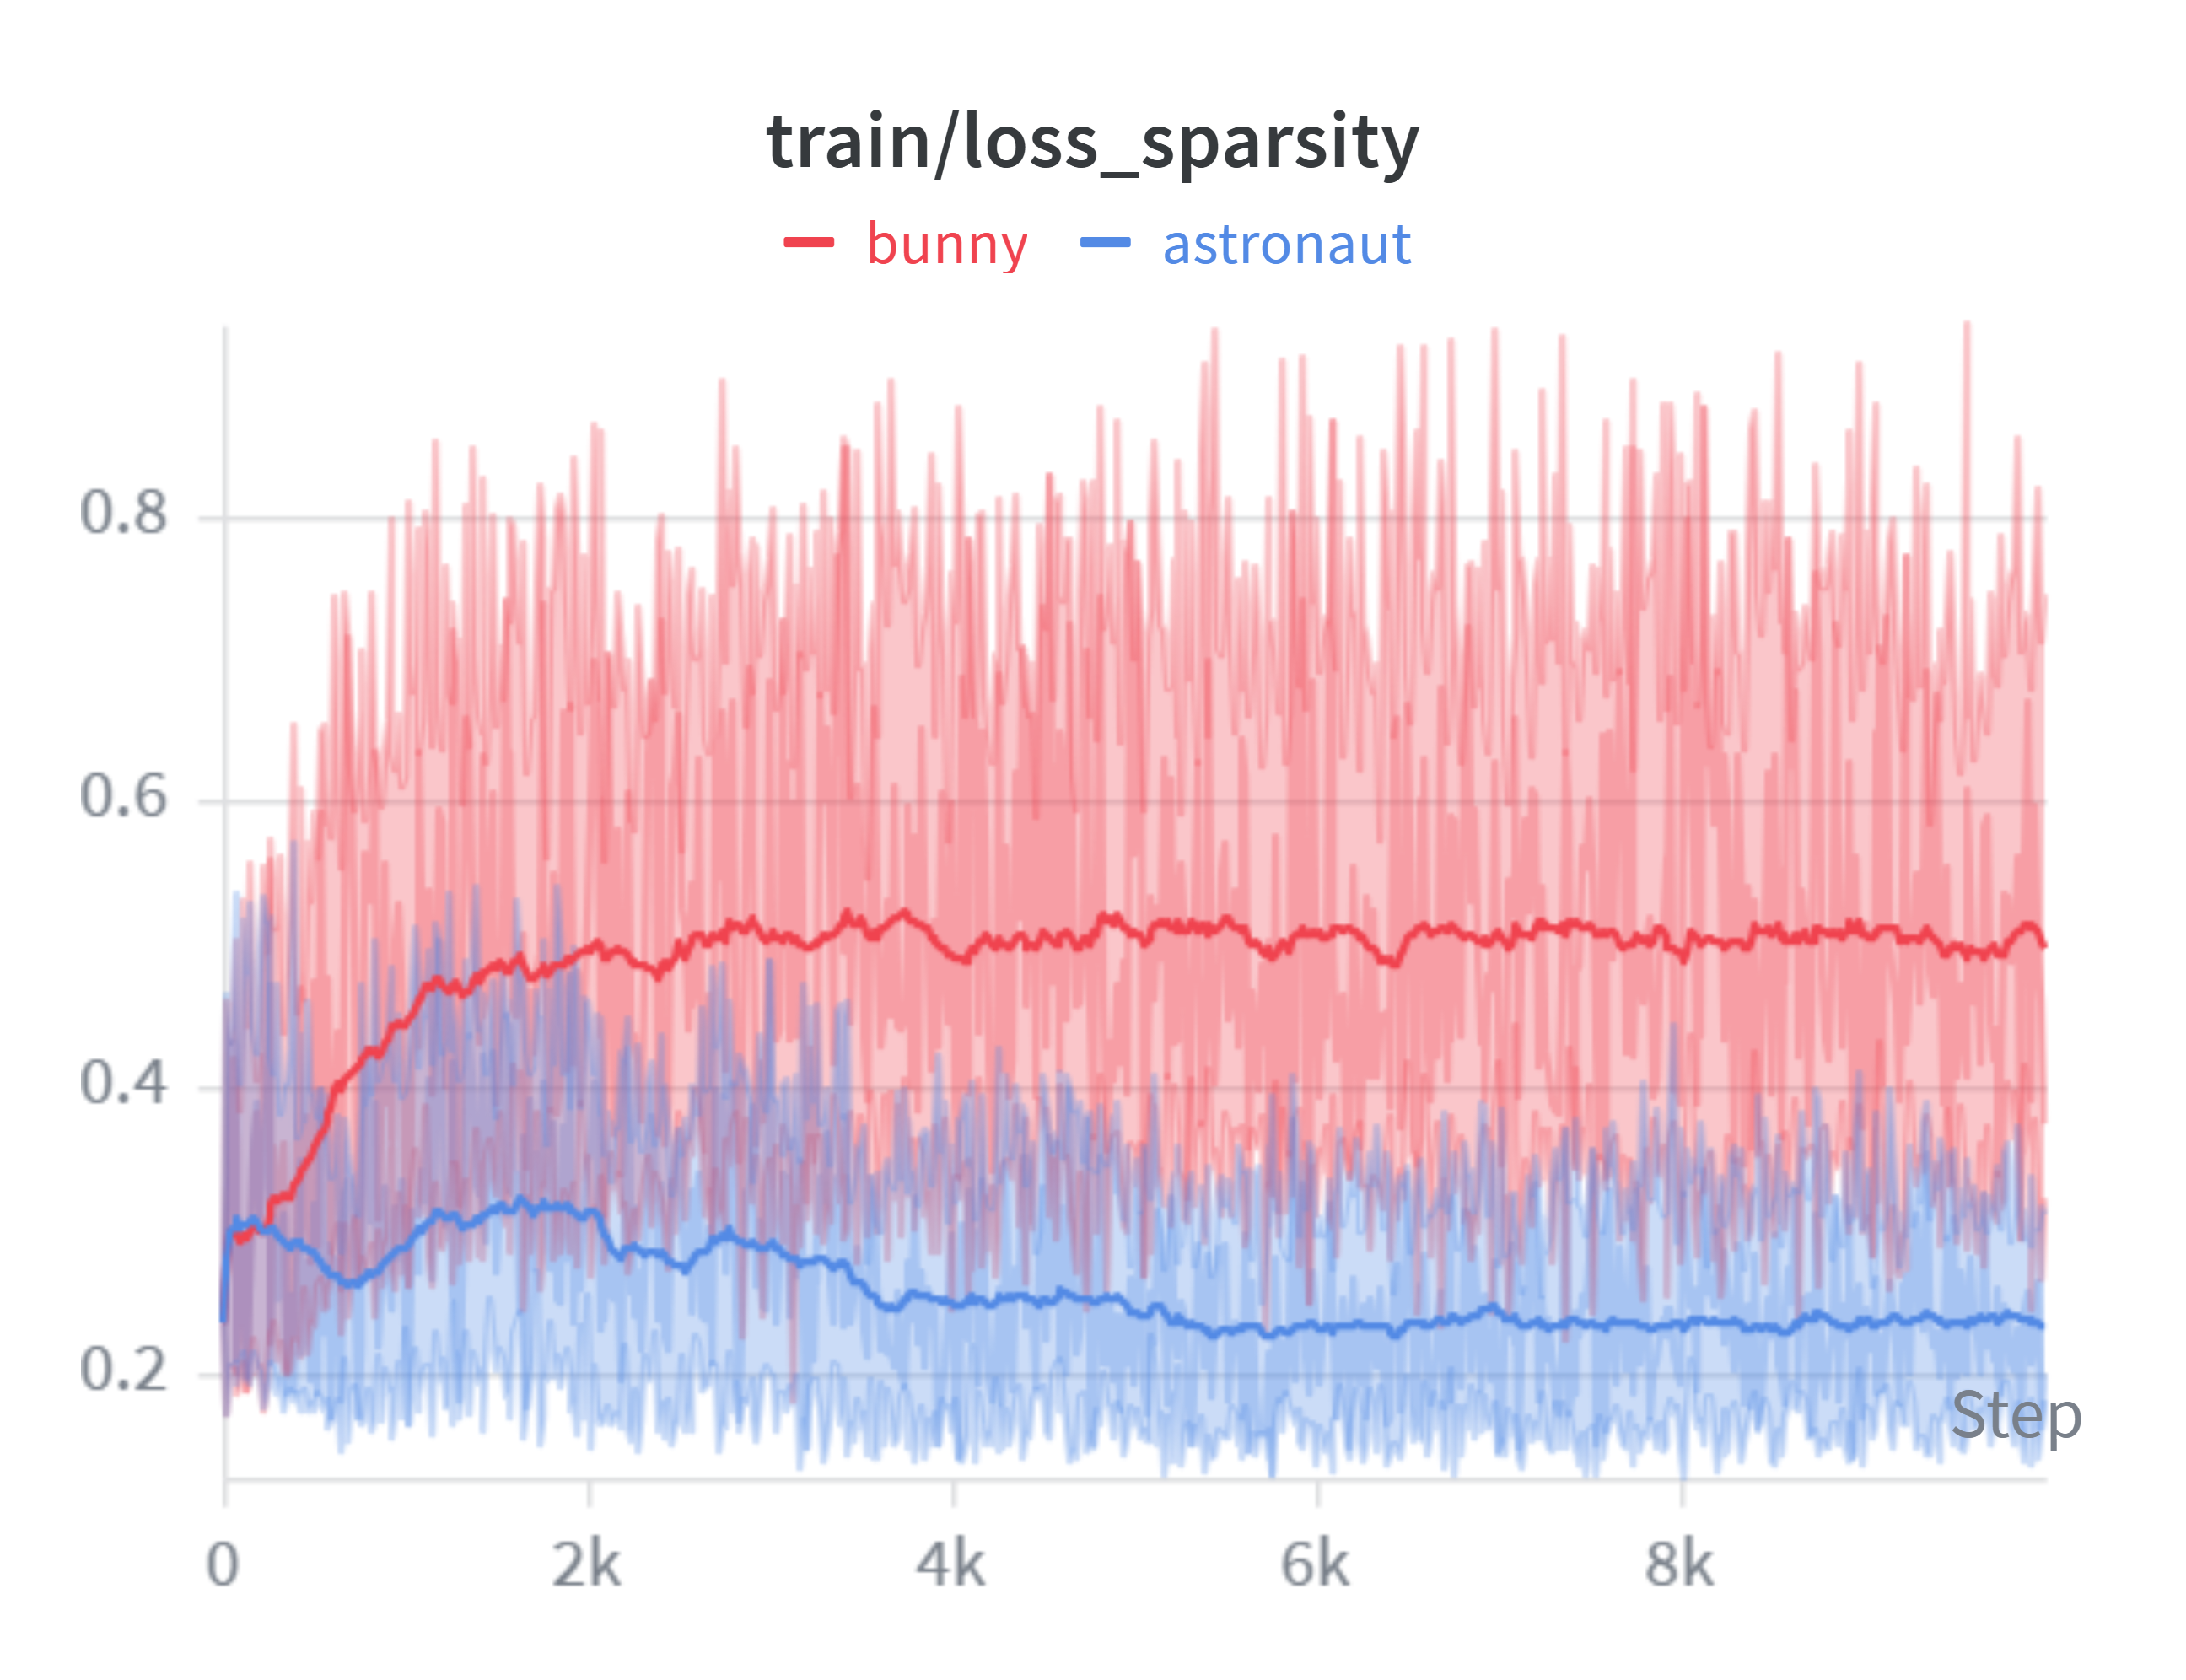
\includegraphics[width=\linewidth]{figures/task1/objectB/sparsity_loss.png}
		\caption{Sparsity Loss}
	\end{subfigure}
	\hfill
	\begin{subfigure}{0.4\textwidth}
		\centering
		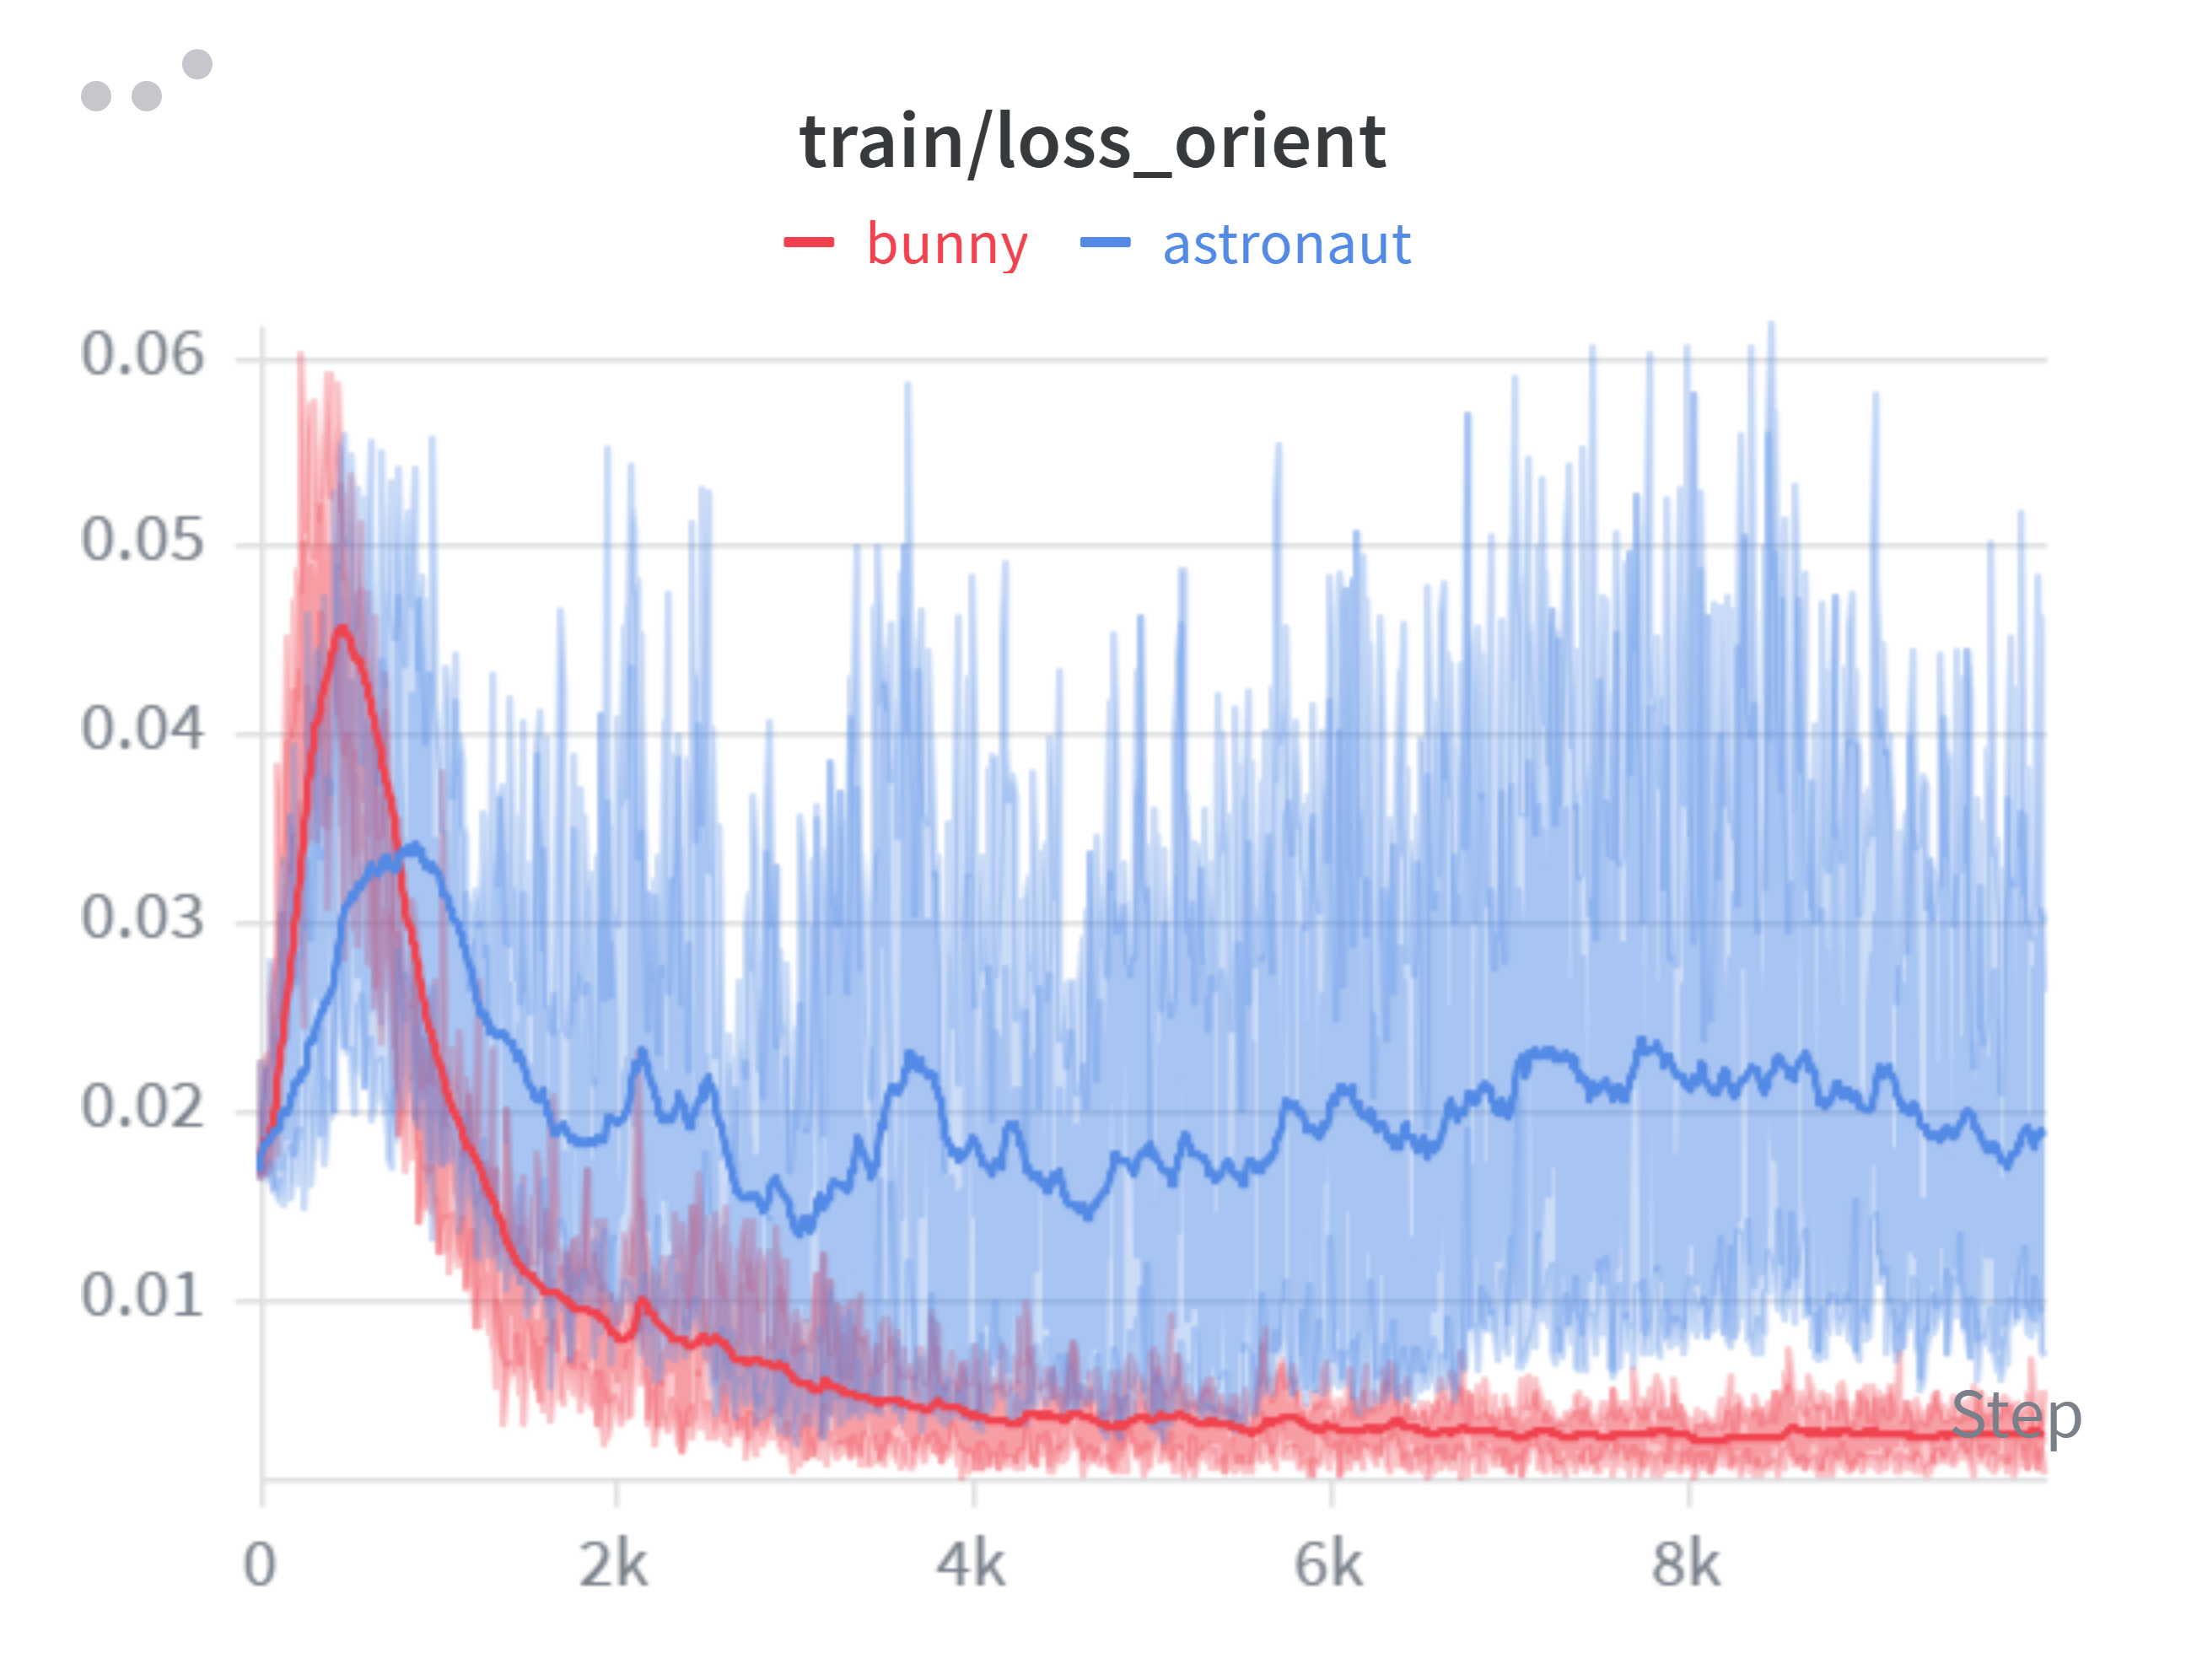
\includegraphics[width=\linewidth]{figures/task1/objectB/orient_loss.png}
		\caption{Orient Loss}
	\end{subfigure}
	
	\caption{Visualization results of generated 3D objects and training loss functions.}
	\label{fig:results_and_losses}
\end{figure}

We can see from the model visualizations that the astronaut has a relatively less smoother outfit and less appropriate color distribution, this may because that the pre-trained model doesn't have enough information compared with the bunny.

As for the training dynamics, here are our analysis:

SDS Loss exhibits extremely large magnitude values, reaching into the thousands, accompanied by very high variance and strong oscillations. Unlike typical supervised learning objectives, it does not demonstrate a smooth and monotonic decreasing trend during optimization. In 3D generative tasks, SDS Loss is derived from a pretrained diffusion model and fundamentally provides gradient directions in the parameter space rather than serving as an absolute scalar objective to be minimized to zero. Therefore, this behavior is ordinary. Comparing the two objects, the Bunny (red curve) shows significantly higher baseline values and variance than the Astronaut (blue curve), suggesting that the diffusion model provides more uncertain or higher-variance gradient guidance for the Bunny, possibly due to a more complex and unsmooth structure of the astronaut.

Opaque Loss decreases rapidly during the early stages of training and then gradually approaches a stable asymptotic plateau. This loss typically acts as a regularization term that removes floating artifacts and encourages the model to produce solid geometry. The Bunny converges very quickly and stabilizes near zero with minimal noise, whereas the Astronaut also decreases but eventually stabilizes at a relatively higher mean value (approximately 0.05 to 0.1) and retains noticeable variance in later stages. This indicates that the Astronaut presents a more challenging optimization landscape for opacity regularization.But the total structure is still clear.

Sparsity Loss increases rapidly in the early training stage before entering a highly oscillatory plateau. This reflects the constraint on spatial occupancy, encouraging empty space outside the object region. The initial increase indicates that the model is expanding its occupied volume while constructing the coarse geometry, while the subsequent plateau reflects a dynamic equilibrium between forming complete structures and maintaining spatial sparsity. The Bunny stabilizes at a relatively higher level (around 0.5), while the Astronaut stabilizes at a lower value (around 0.2). Suggesting that the Bunny occupies a more spatially extensive or volumetrically dense structure, resulting in higher sparsity penalties,which is aligned with the visualization results.

Orient Loss demonstrates a characteristic “spike-then-decay” behavior. This loss is typically used to regularize surface normals, ensuring smooth and physically consistent surface orientations while preventing jagged artifacts. The initial spike occurs when the model begins forming its coarse geometry and surface normals are highly disordered. As training progresses and the geometry becomes smoother, the loss decreases and converges. The Bunny reaches its peak around 1000 steps and then converges smoothly toward near-zero values, indicating highly optimized surface smoothness. In contrast, the Astronaut peaks slightly earlier but retains higher fluctuations and a non-negligible residual value (around 0.02), suggesting that its surface geometry is more complex.








\subsubsection{Object C}
In this section, the following picture is trained:

\begin{figure}[H]
	\centering
	
	% 第一张图（左边）
	\begin{subfigure}{0.4\textwidth}
		\centering
		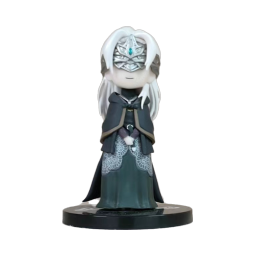
\includegraphics[width=\linewidth]{figures/task1/objectC/firekeeper_rgba.png} % 第一张图片路径
		\caption{Firekeeper(threestudio)}
	\end{subfigure}
	\hfill % 两张图之间的间距
	% 第二张图（右边）
	\begin{subfigure}{0.4\textwidth}
		\centering
		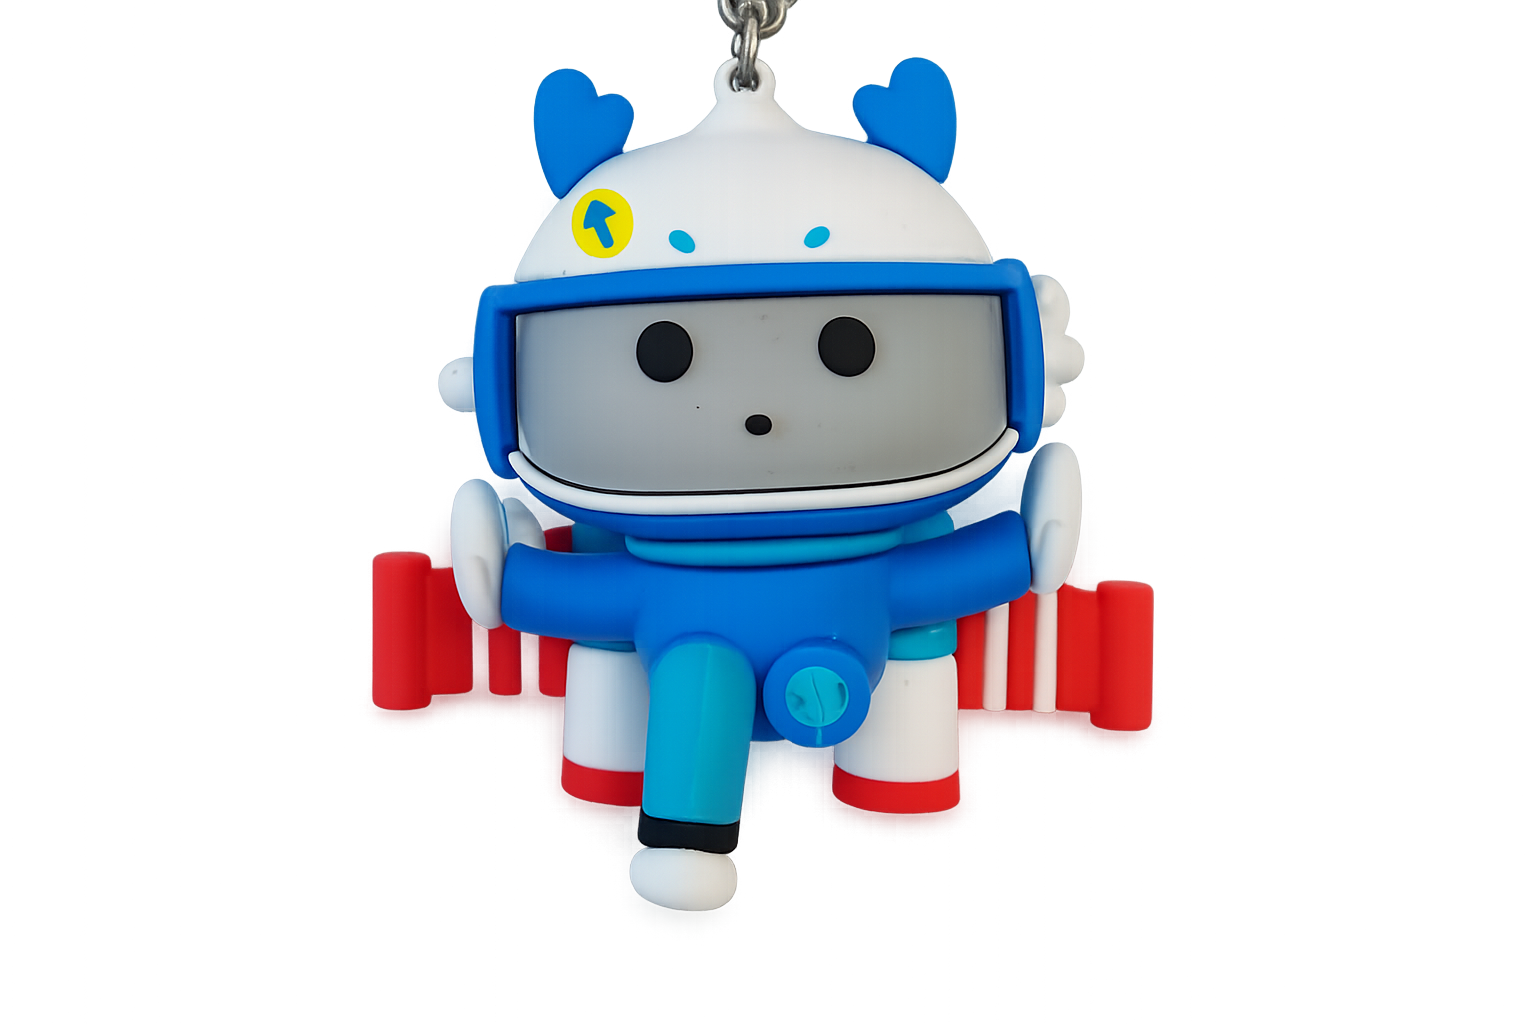
\includegraphics[width=\linewidth]{figures/task1/objectC/cute_robot_rgba.png} % 替换为你的第二张图片路径
		\caption{Cute Astronaut Robot(Ours)}
	\end{subfigure}

\end{figure}


Each training takes about \textbf{30min}(coarse)+\textbf{30min}(refine), the rendering results and training dynamics are as follow:

\begin{figure}[H]
	\centering
	
	%================ 第一组：Astronaut =================
	\begin{subfigure}{0.25\textwidth}
		\centering
		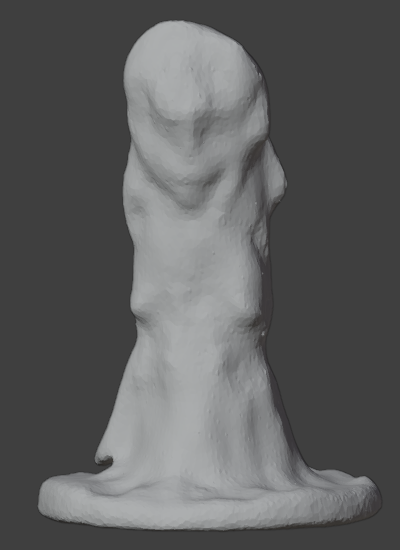
\includegraphics[width=\linewidth]{figures/task1/objectC/firekeeper_mesh.png}
		\caption{Firekeeper Mesh}
	\end{subfigure}
	\hfill
	\begin{subfigure}{0.25\textwidth}
		\centering
		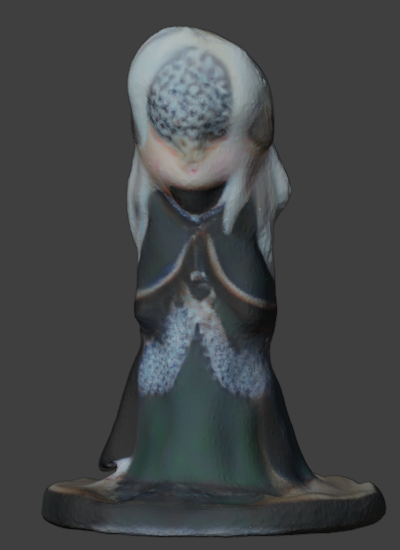
\includegraphics[width=\linewidth]{figures/task1/objectC/firekeeper_color.png}
		\caption{Firekeeper Color}
	\end{subfigure}
	\hfill
	\begin{subfigure}{0.25\textwidth}
		\centering
		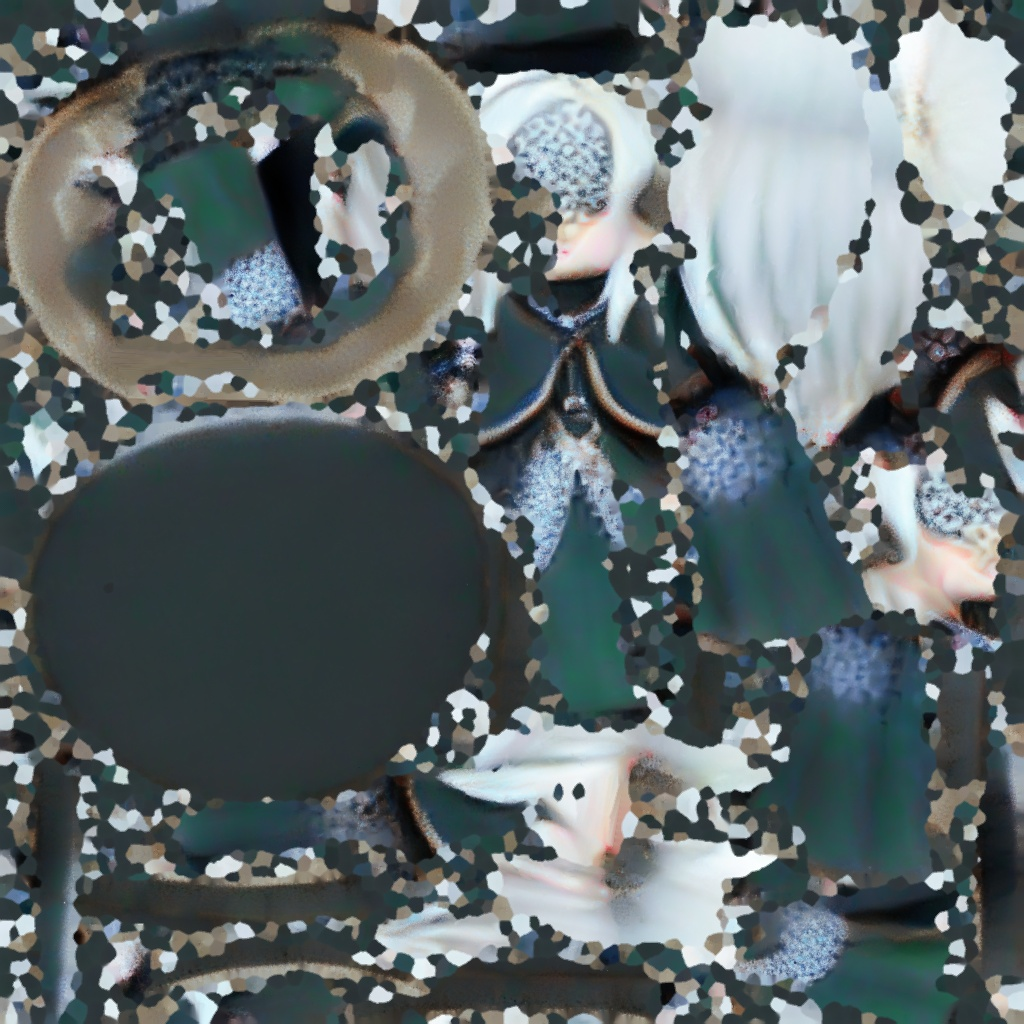
\includegraphics[width=\linewidth]{figures/task1/objectC/firekeeper_texture_kd.jpg}
		\caption{Firekeeper Texture}
	\end{subfigure}
	
	
\end{figure}




\begin{figure}[H]
	\centering
	
	% 第一张
	
\includegraphics[width=0.6\textwidth]{figures/task1/objectC/firekeeper1.png} % 替换为你的实际路径

	
	\vspace{0.3cm} % 调整图片之间的垂直间距
	
	% 第二张
	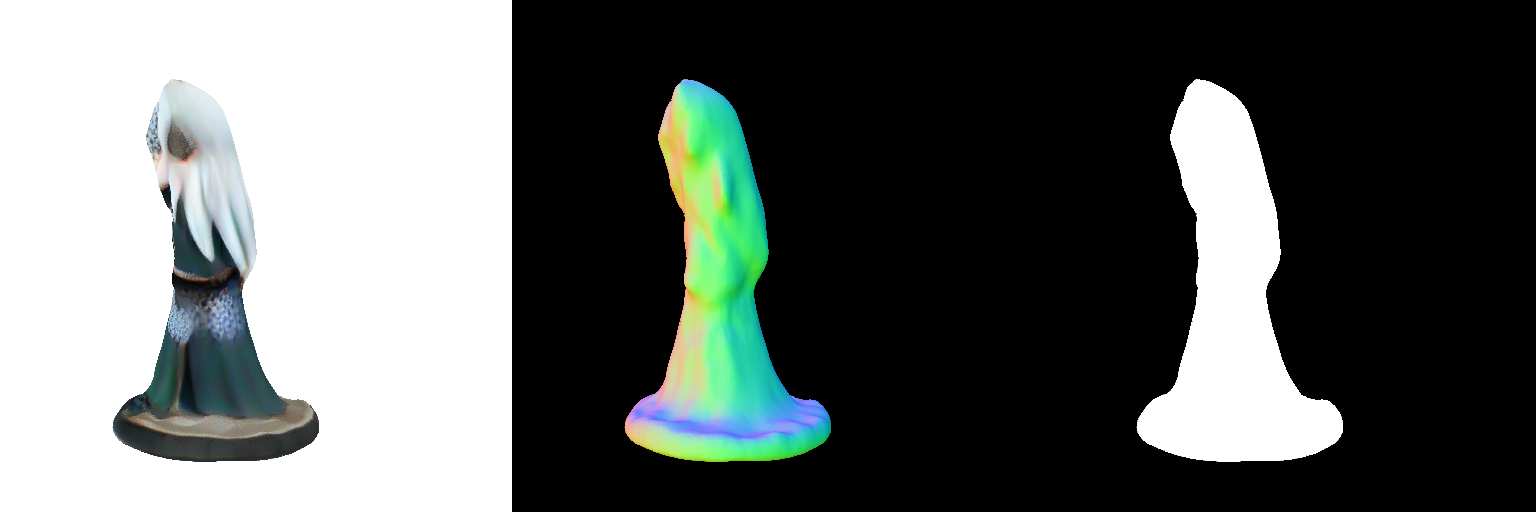
\includegraphics[width=0.6\textwidth]{figures/task1/objectC/firekeeper2.png}

	
	\vspace{0.3cm}
	
	% 第三张
	
\includegraphics[width=0.6\textwidth]{figures/task1/objectC/firekeeper3.png}

	
	\vspace{0.3cm}
	
	% 第四张
	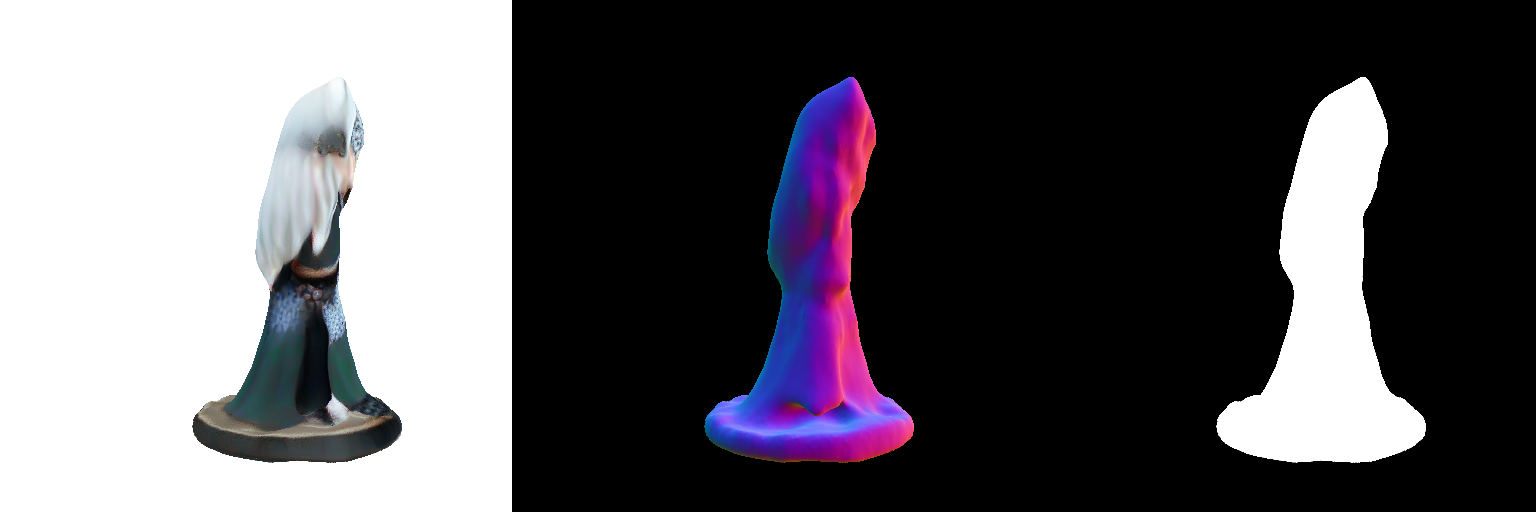
\includegraphics[width=0.6\textwidth]{figures/task1/objectC/firekeeper4.png}

	
	\caption{Different Viewpoints}
	\label{fig:firekeeper_vertical}
\end{figure}

\begin{figure}[H]
		\begin{subfigure}{0.25\textwidth}
		\centering
		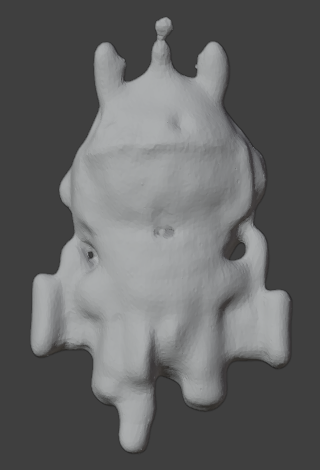
\includegraphics[width=\linewidth]{figures/task1/objectC/cute_robot_mesh.png}
		\caption{Robot Mesh}
	\end{subfigure}
	\hfill
	\begin{subfigure}{0.25\textwidth}
		\centering
		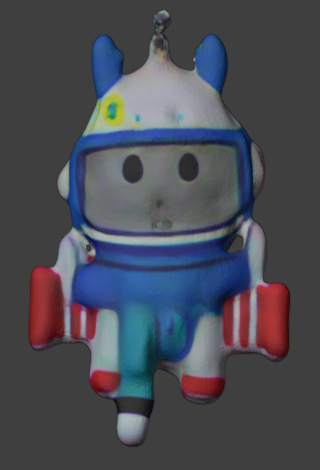
\includegraphics[width=\linewidth]{figures/task1/objectC/cute_robot_color.png}
		\caption{Robot Color}
	\end{subfigure}
	\hfill
	\begin{subfigure}{0.25\textwidth}
		\centering
		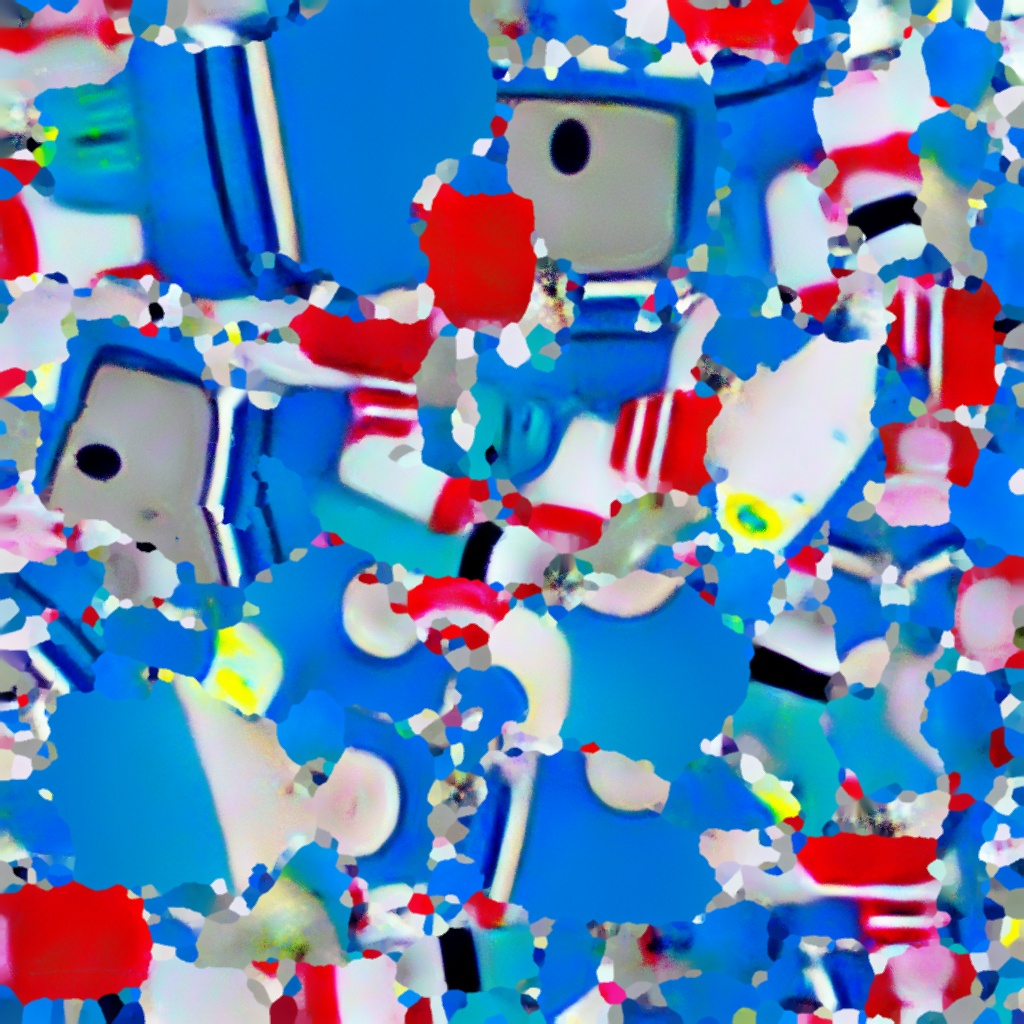
\includegraphics[width=\linewidth]{figures/task1/objectC/robot_texture_kd.jpg}
		\caption{Robot Texture}
	\end{subfigure}
\end{figure}

\begin{figure}[H]
	\centering
	
	% 第一张
	
\includegraphics[width=0.6\textwidth]{figures/task1/objectC/robot1.png} % 替换为你的实际路径
	
	
	\vspace{0.3cm} % 调整图片之间的垂直间距
	
	% 第二张
	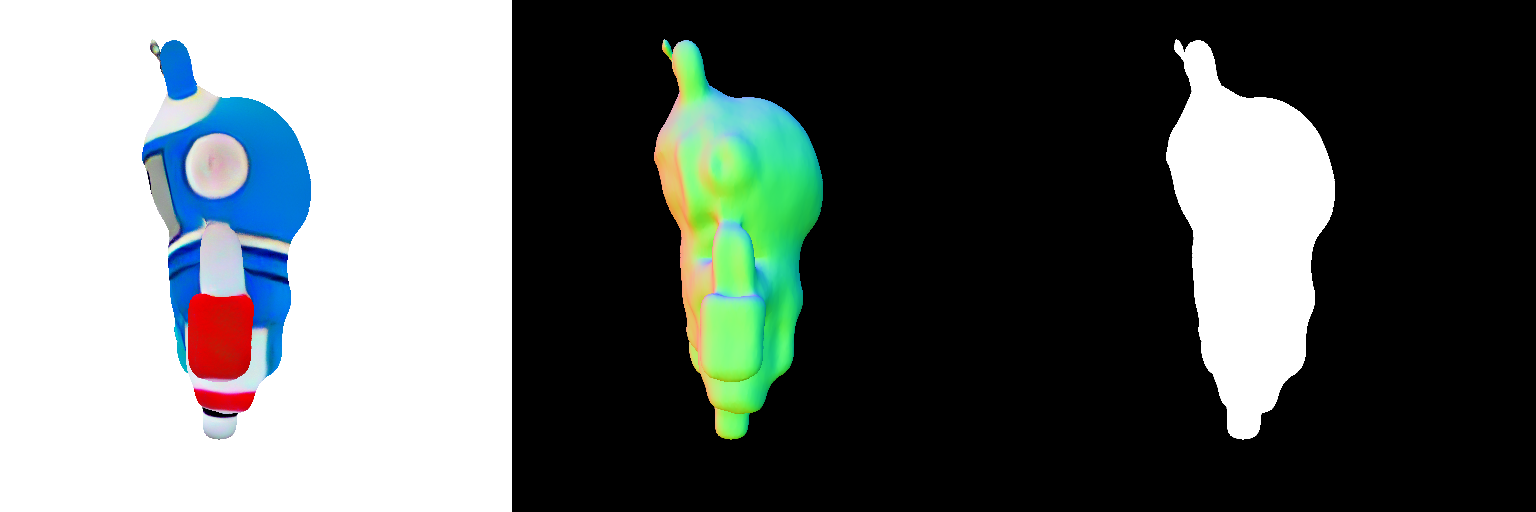
\includegraphics[width=0.6\textwidth]{figures/task1/objectC/robot2.png}
	
	
	\vspace{0.3cm}
	
	% 第三张
	
\includegraphics[width=0.6\textwidth]{figures/task1/objectC/robot3.png}
	
	
	\vspace{0.3cm}
	
	% 第四张
	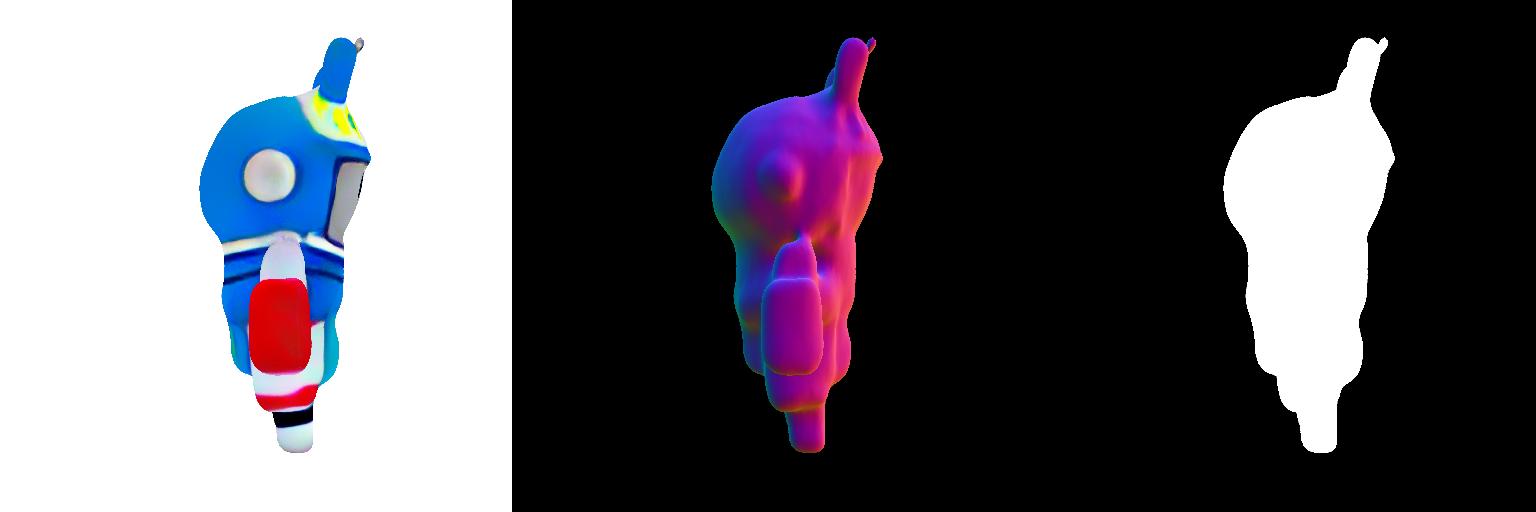
\includegraphics[width=0.6\textwidth]{figures/task1/objectC/robot4.png}
	
	
	\caption{Different Viewpoints}
	\label{fig:Robot_vertical}
\end{figure}



\begin{figure}[H]
	\centering
	
	% 第一张图（左边）
	\begin{subfigure}{0.48\textwidth}
		\centering
		
\includegraphics[width=\linewidth]{figures/task1/objectC/opaque_loss.png} % 第一张图片路径
		\caption{Firekeeper(threestudio)}
	\end{subfigure}
	\hfill % 两张图之间的间距
	% 第二张图（右边）
	\begin{subfigure}{0.48\textwidth}
		\centering
		
\includegraphics[width=\linewidth]{figures/task1/objectC/sparsity_loss.png} % 替换为你的第二张图片路径
		\caption{Cute Astronaut Robot(Ours)}
	\end{subfigure}
	
\end{figure}


\begin{figure*}[H]
	\centering
	
	%==================== 第一组：SDS Loss ====================
	\begin{subfigure}[t]{0.32\textwidth}
		\centering
		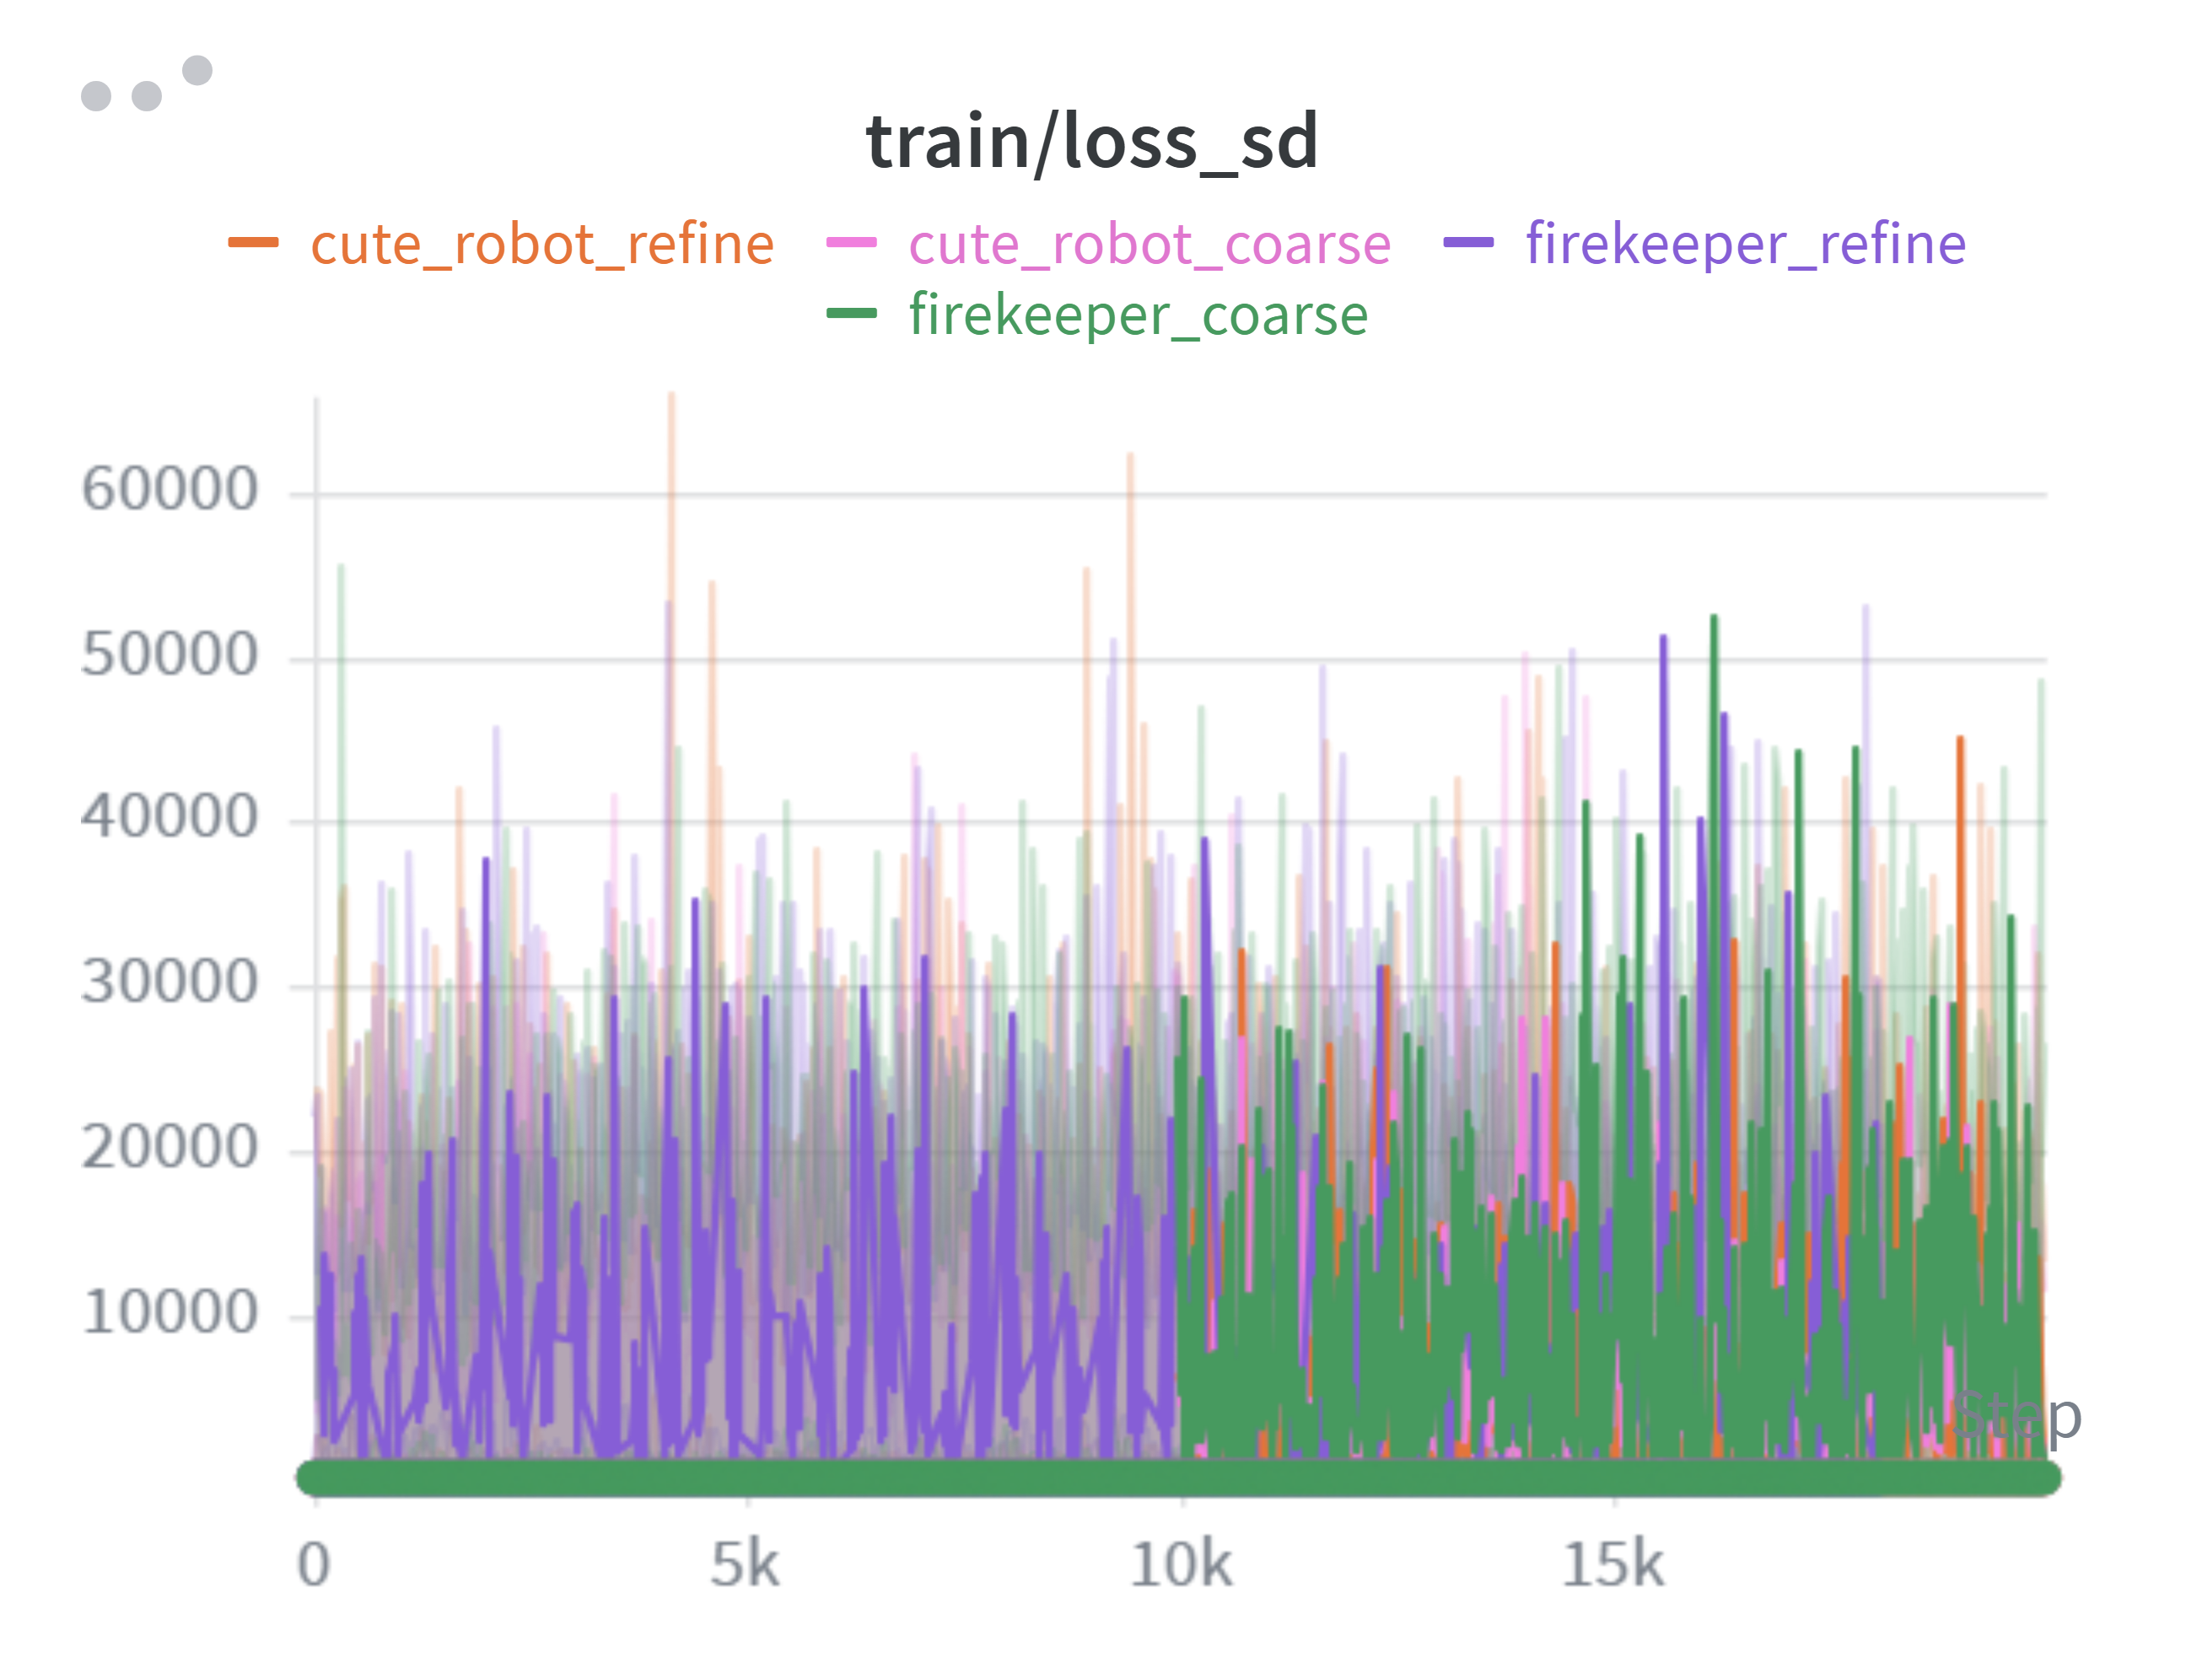
\includegraphics[width=\linewidth]{figures/task1/objectC/losses/loss_sd.png}
		\caption{SDS loss}
	\end{subfigure}
	\hfill
	\begin{subfigure}[t]{0.32\textwidth}
		\centering
		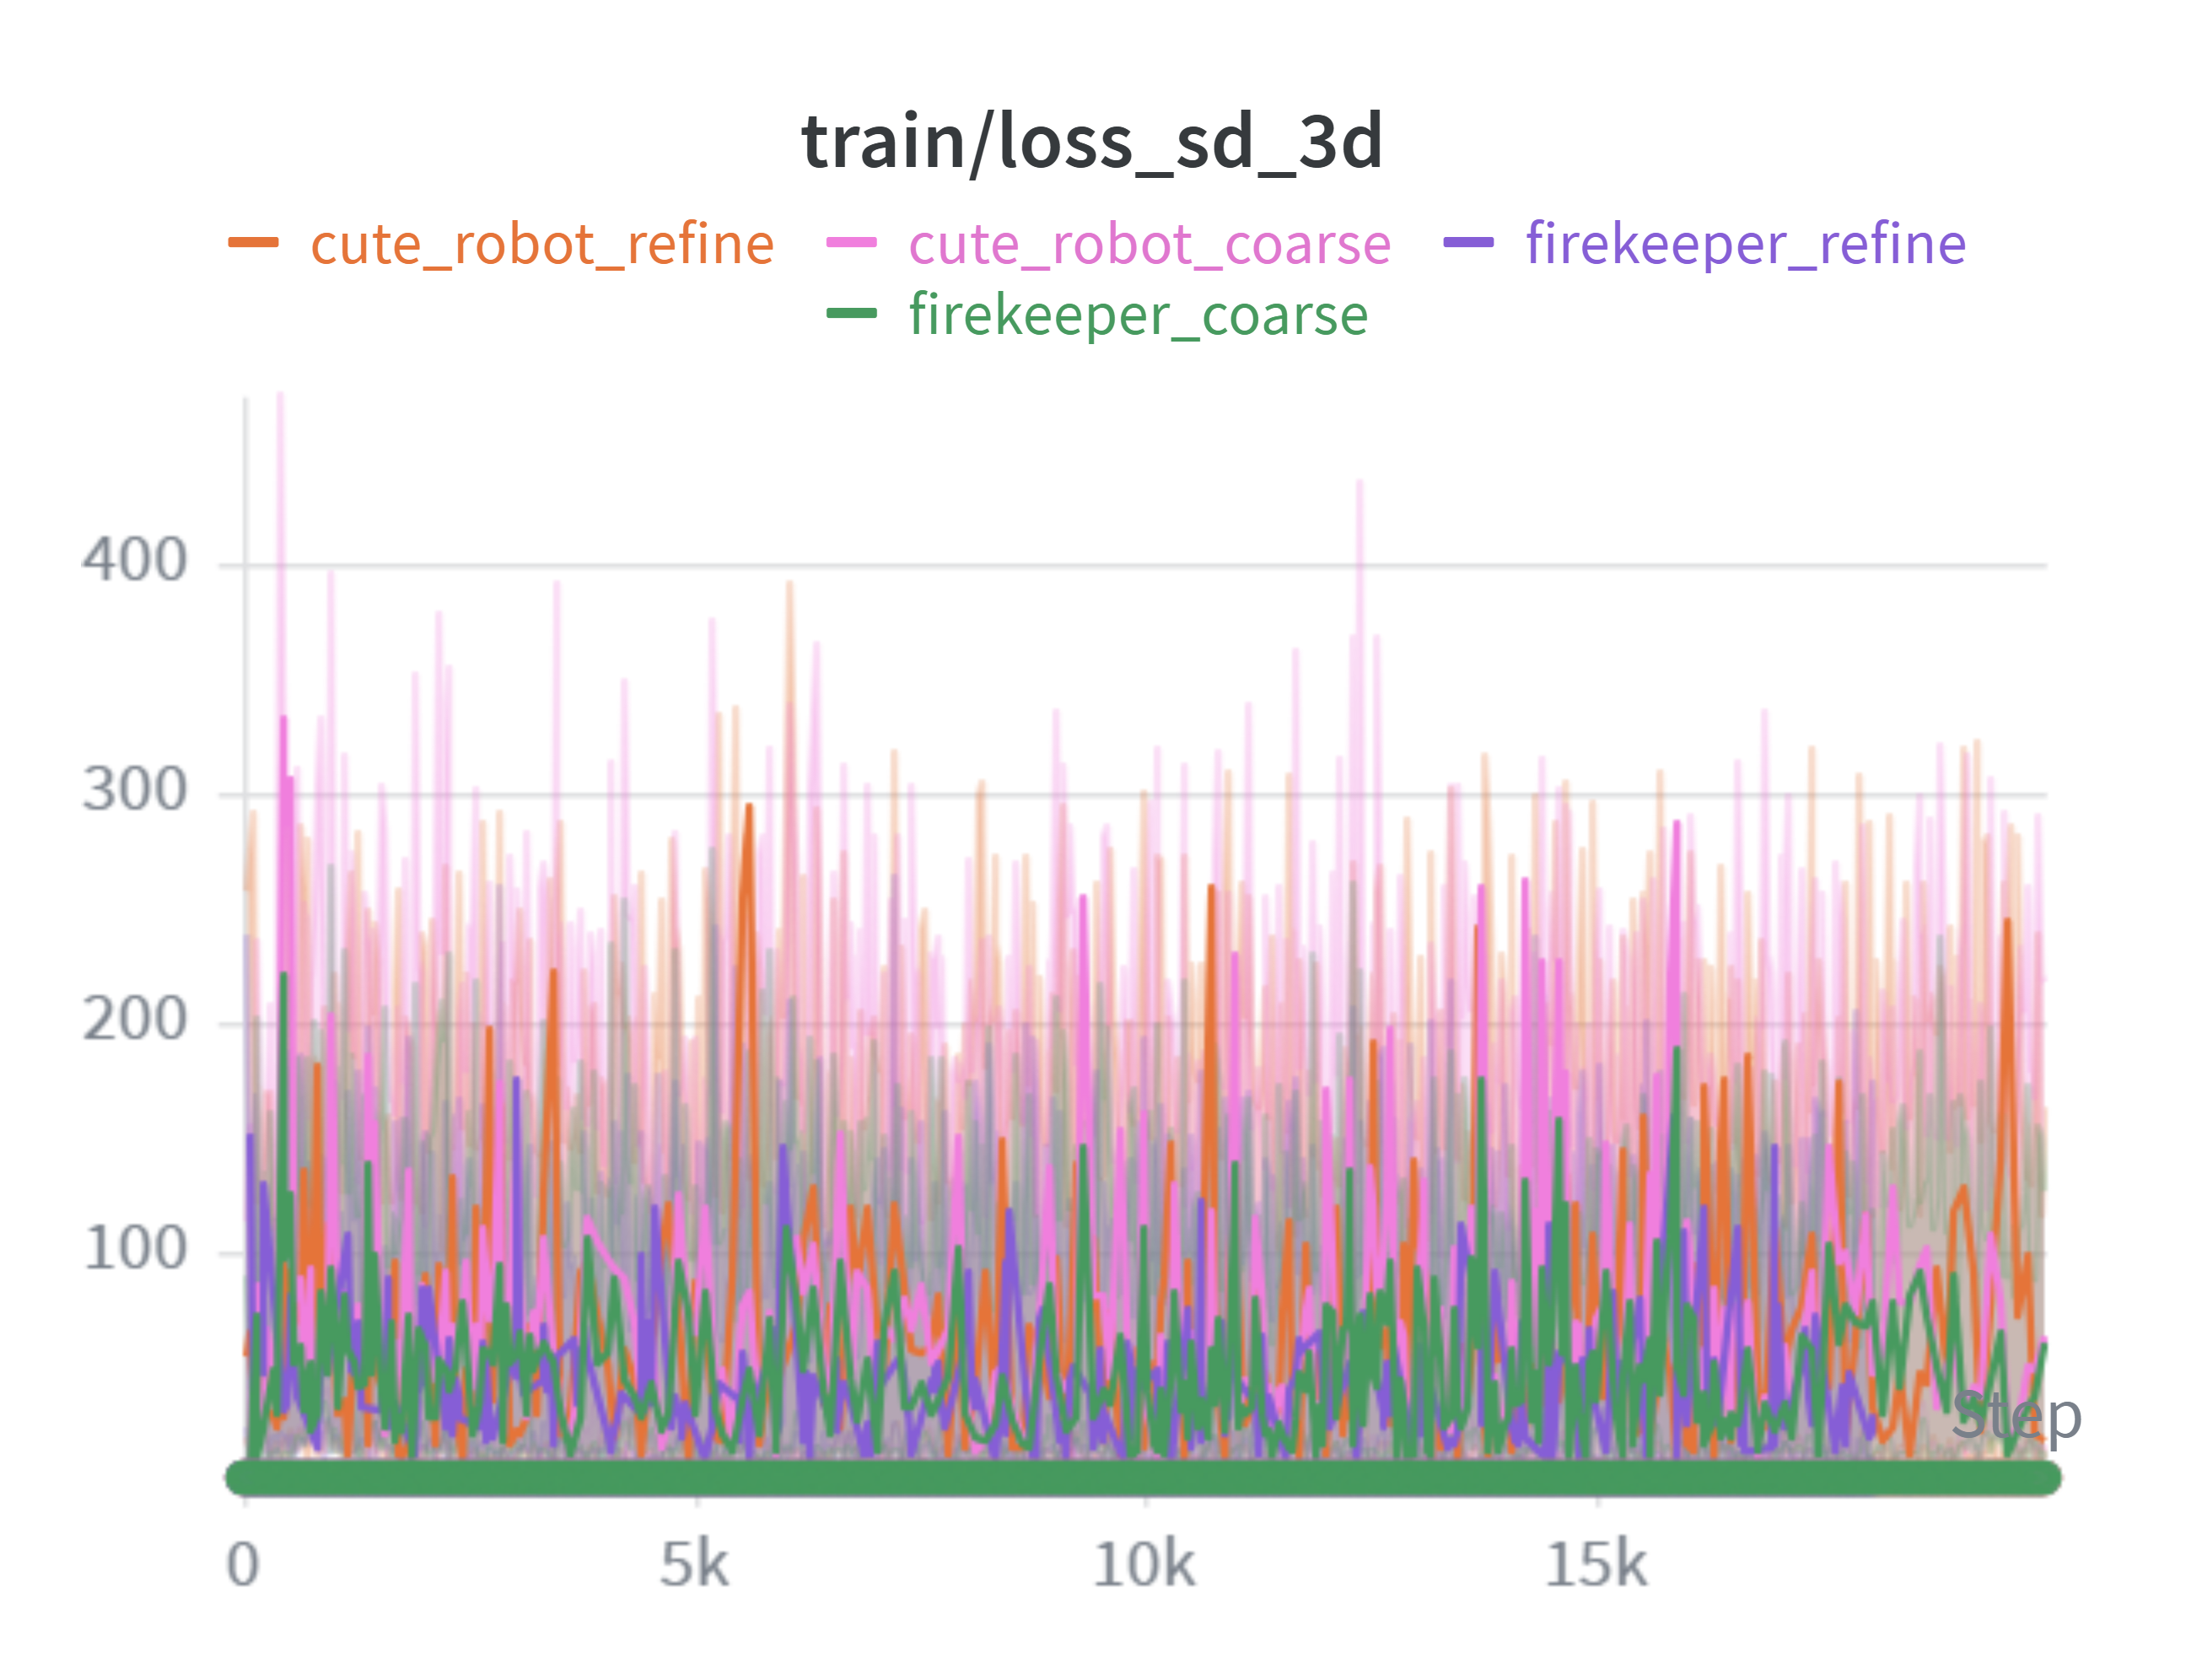
\includegraphics[width=\linewidth]{figures/task1/objectC/losses/loss_sd_3d.png}
		\caption{3D SDS loss}
	\end{subfigure}
	\hfill
	\begin{subfigure}[t]{0.32\textwidth}
		\centering
		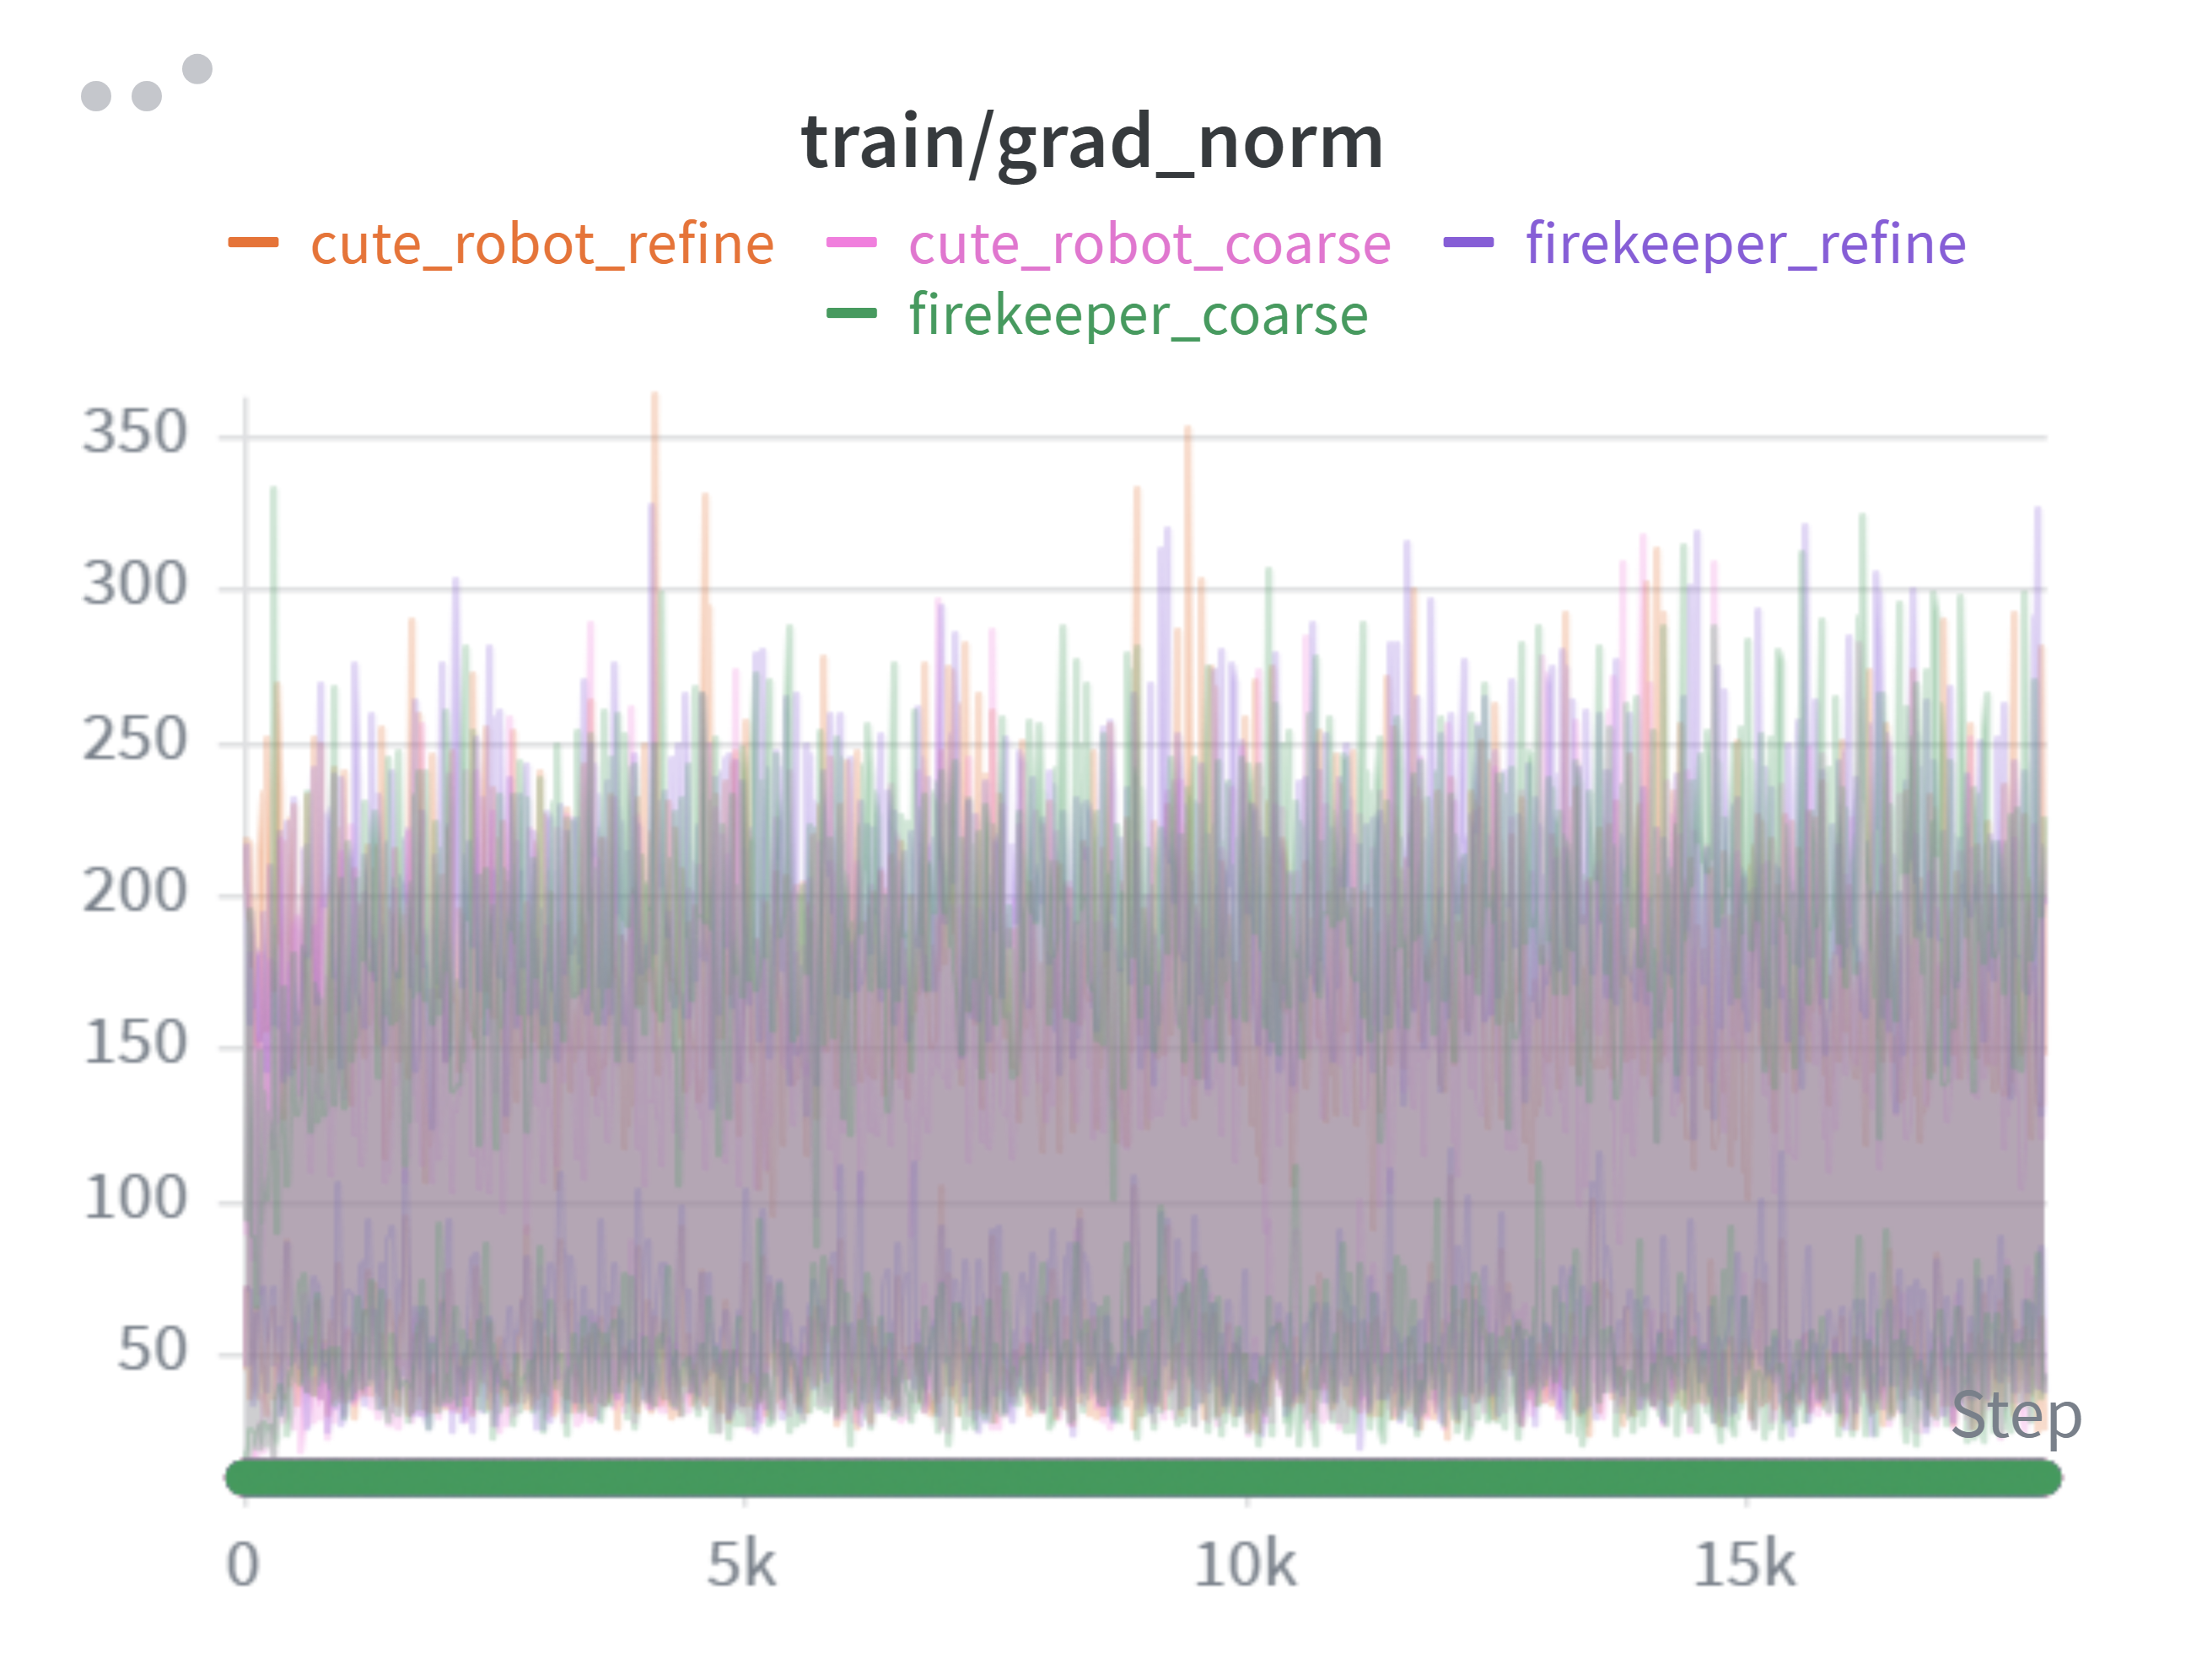
\includegraphics[width=\linewidth]{figures/task1/objectC/losses/grad_norm.png}
		\caption{Gradient norm}
	\end{subfigure}
	
	\vspace{0.5cm}
	
	%==================== 第二组：Regularization ====================
	\begin{subfigure}[t]{0.32\textwidth}
		\centering
		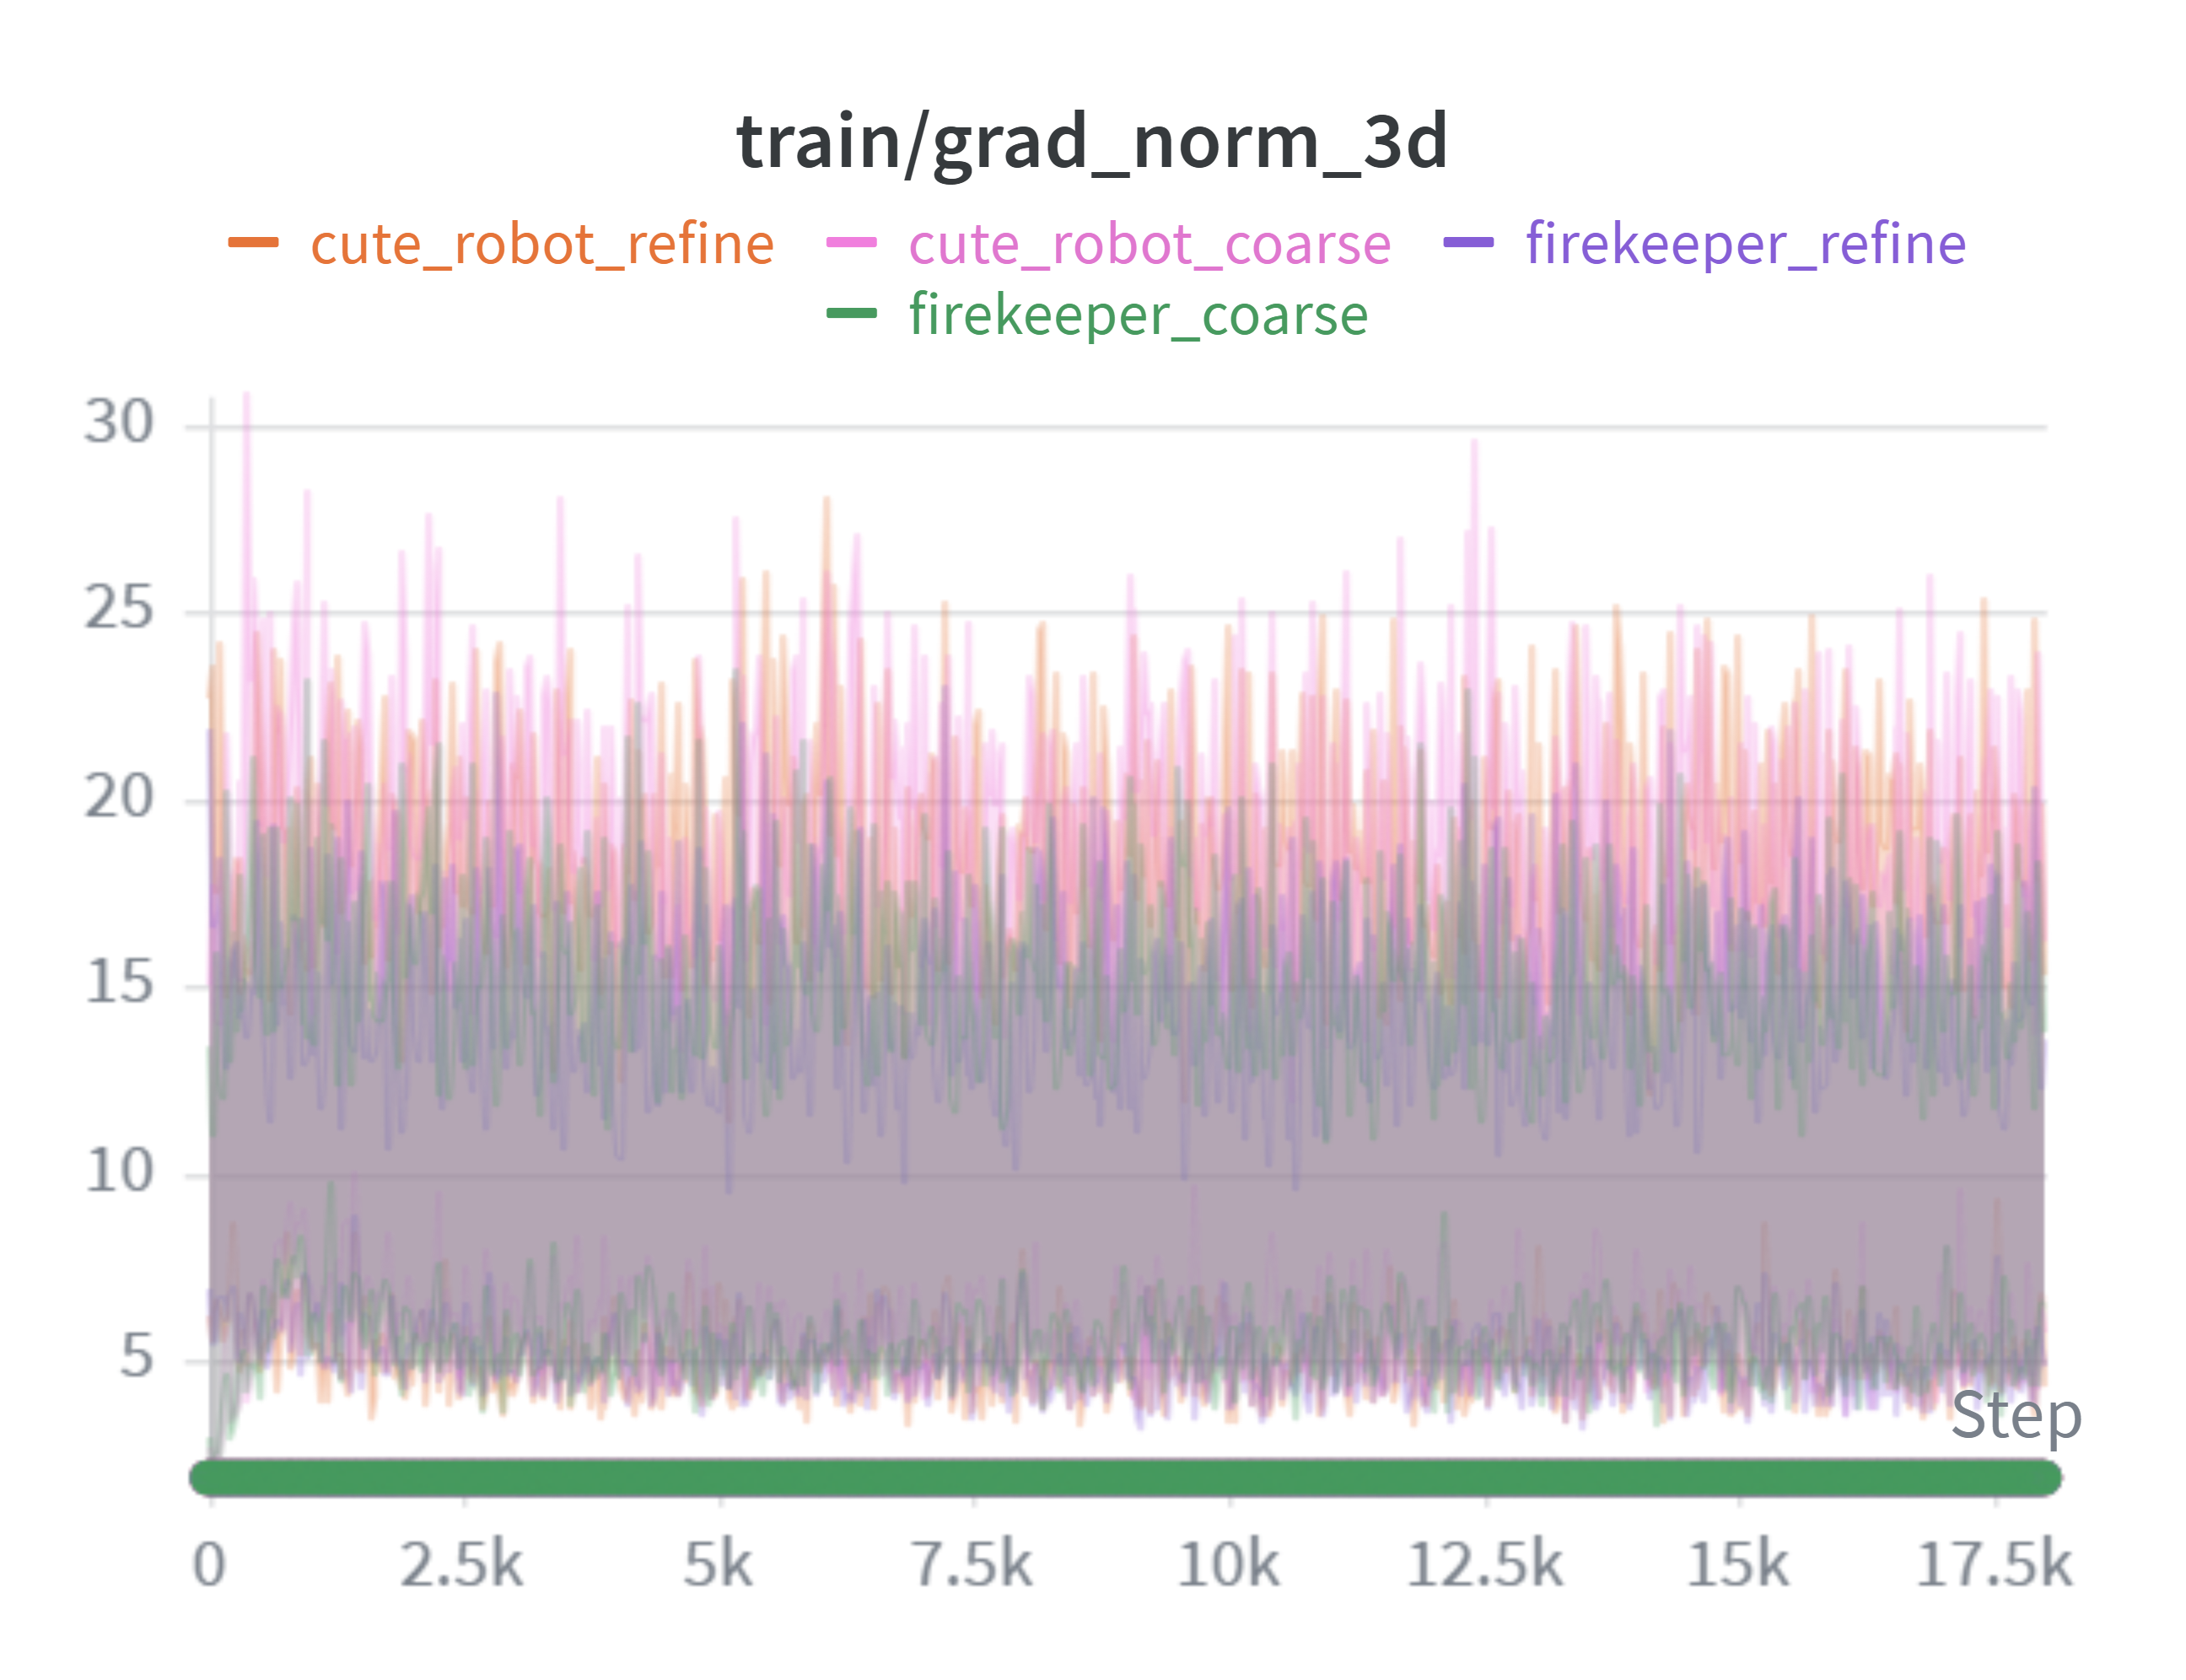
\includegraphics[width=\linewidth]{figures/task1/objectC/losses/grad_norm_3d.png}
		\caption{3D gradient norm}
	\end{subfigure}
	\hfill
	\begin{subfigure}[t]{0.32\textwidth}
		\centering
		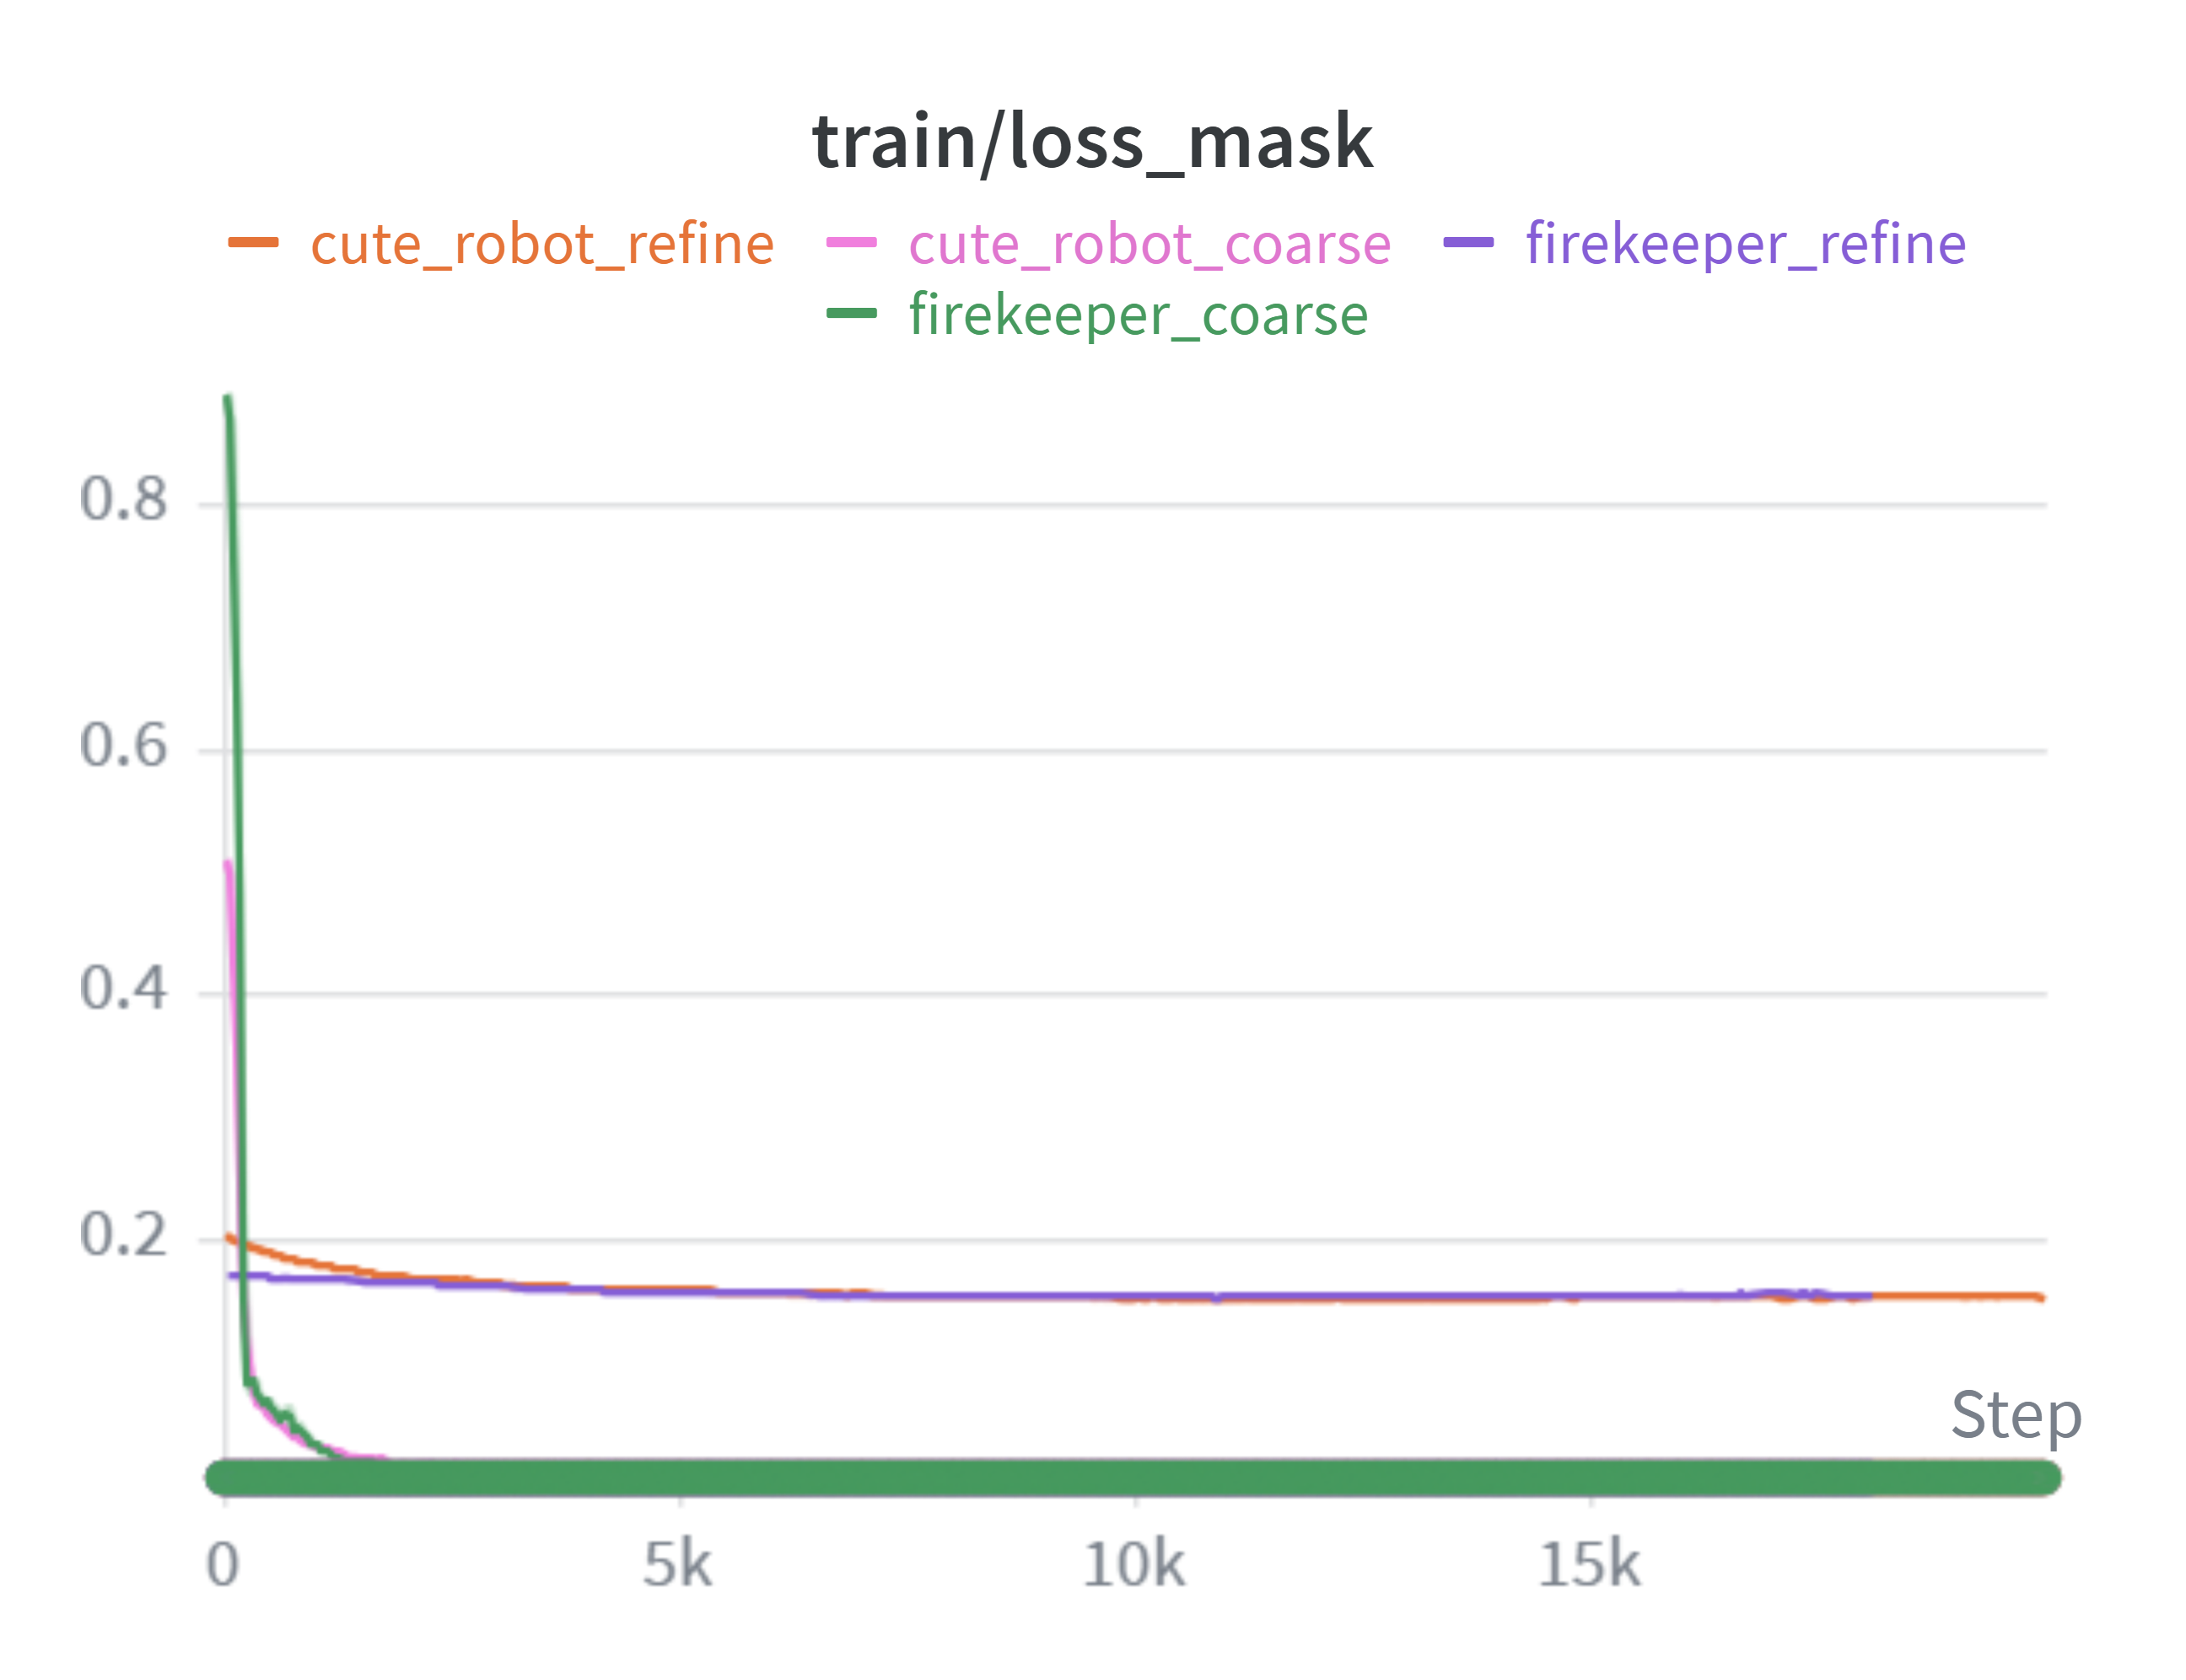
\includegraphics[width=\linewidth]{figures/task1/objectC/losses/loss_mask.png}
		\caption{Mask loss}
	\end{subfigure}
	\hfill
	\begin{subfigure}[t]{0.32\textwidth}
		\centering
		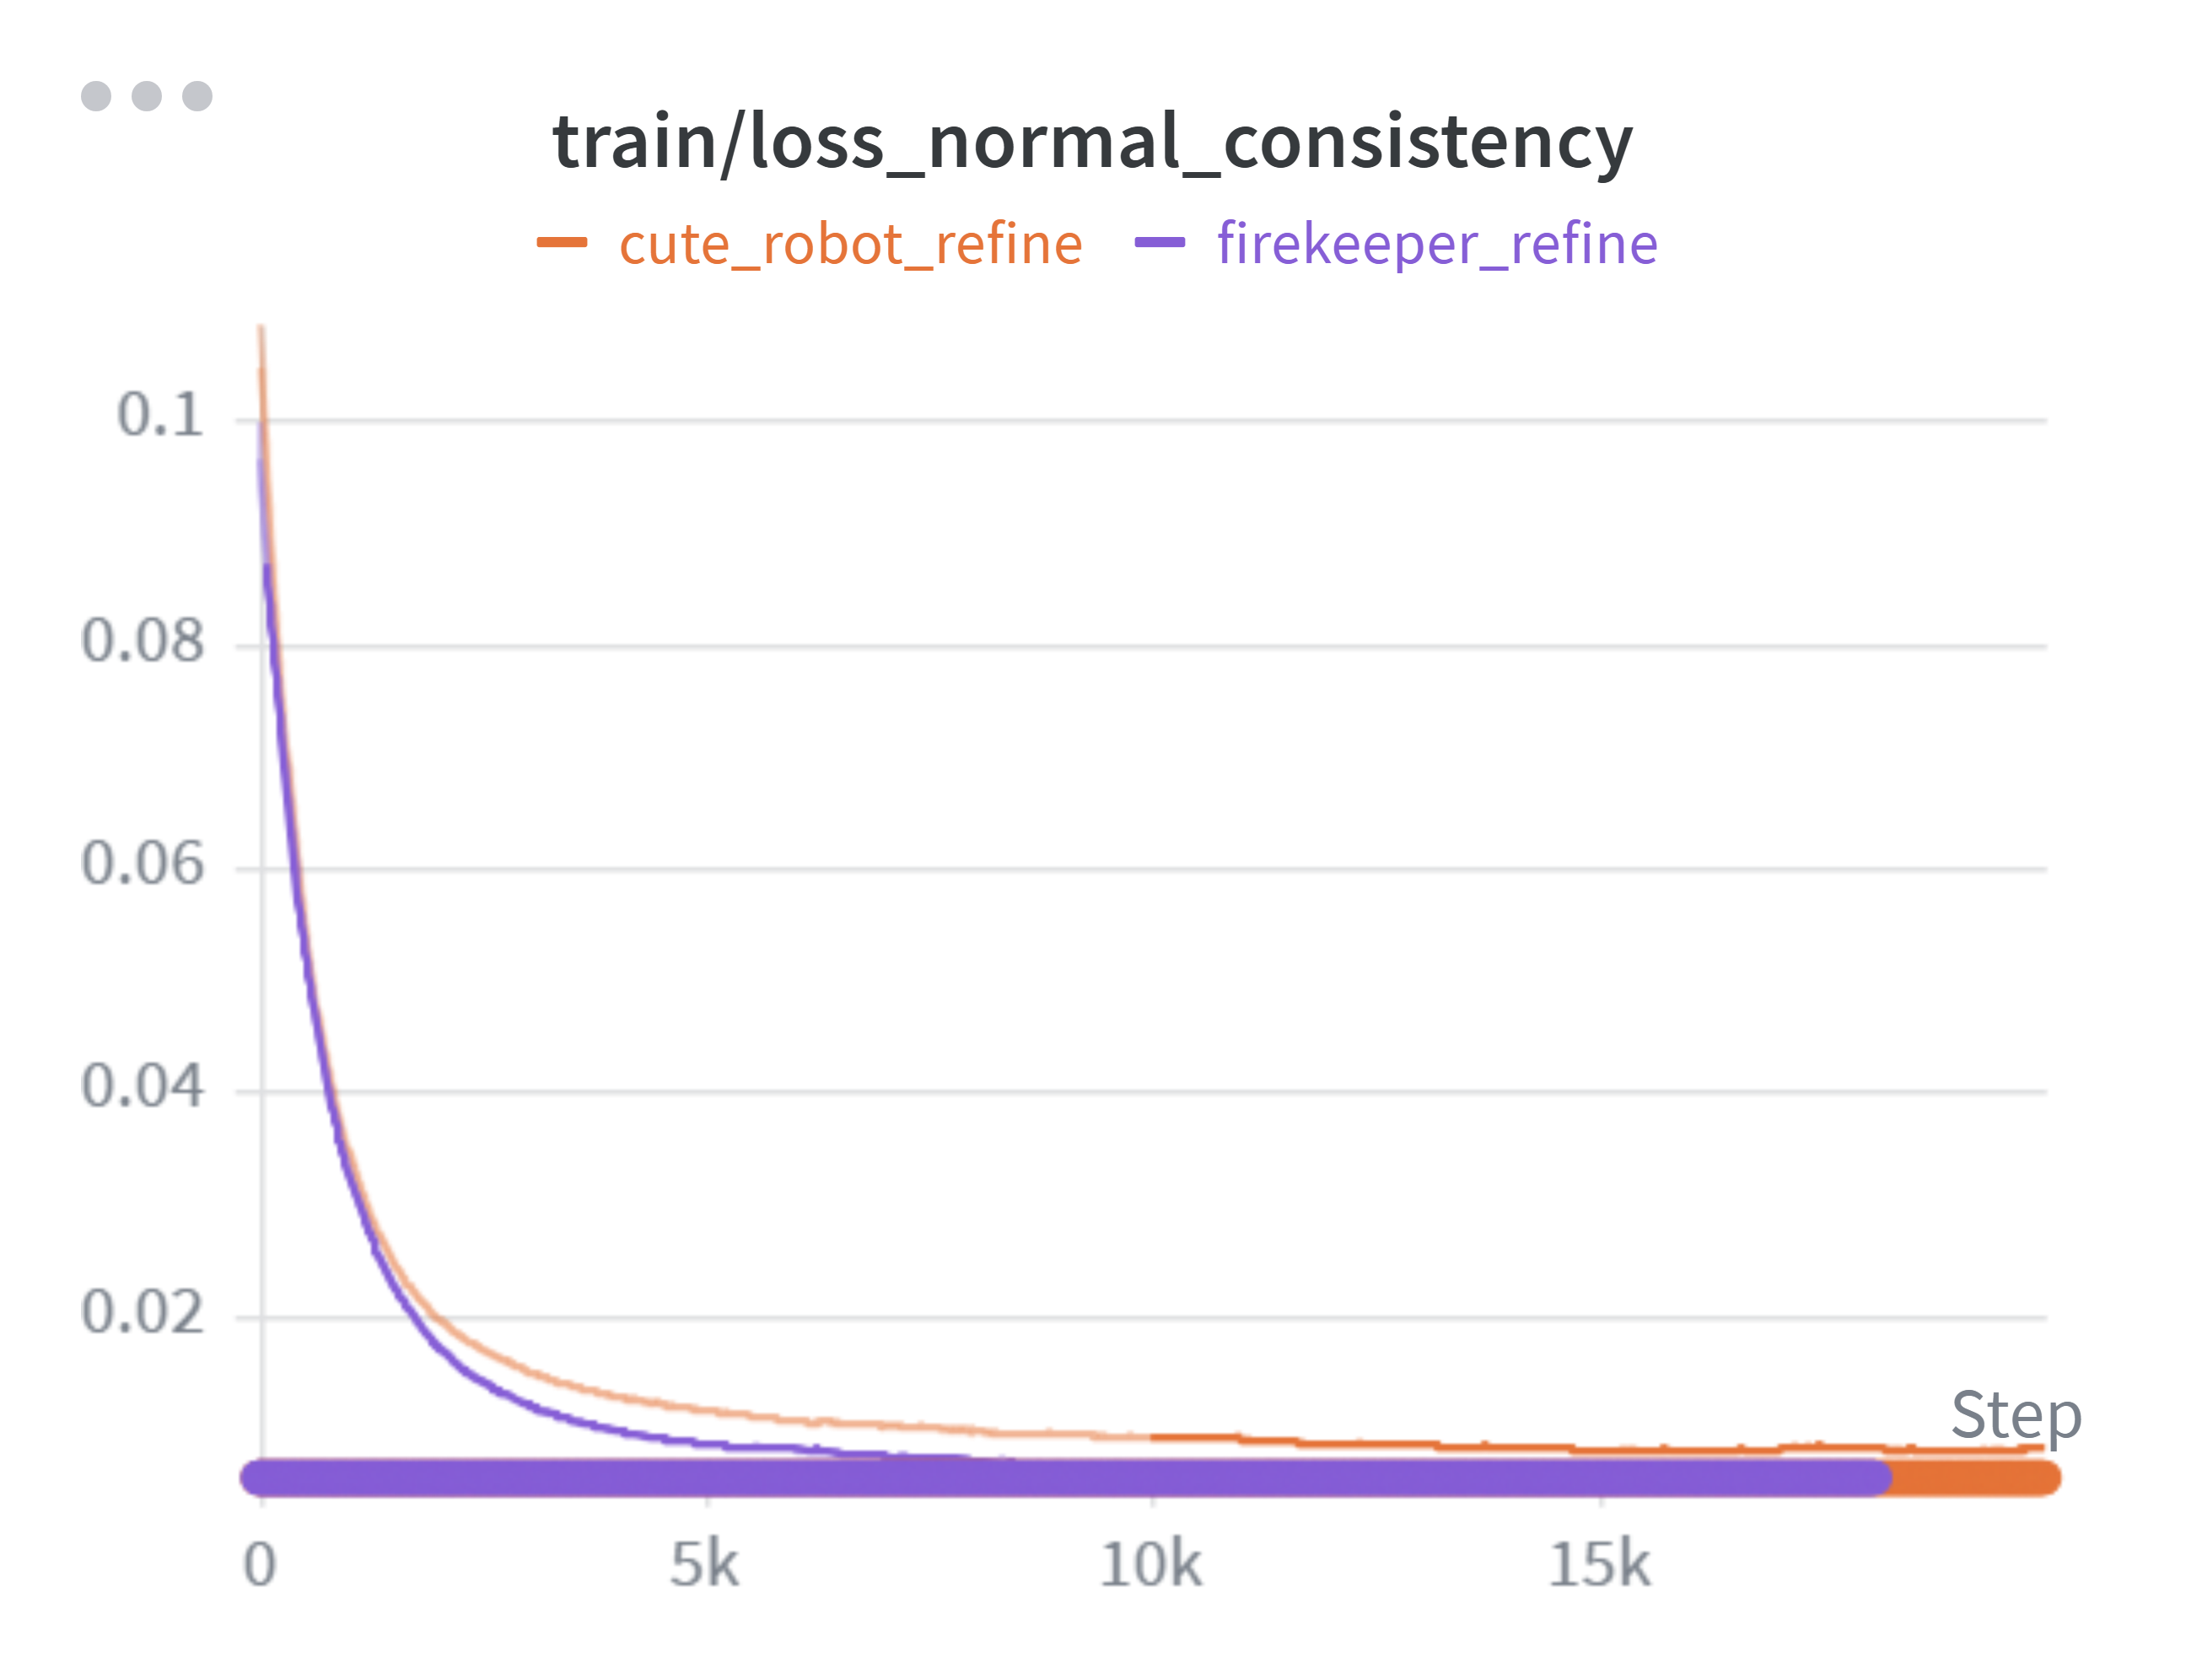
\includegraphics[width=\linewidth]{figures/task1/objectC/losses/loss_normal_consistency.png}
		\caption{Normal consistency loss}
	\end{subfigure}
	
	\vspace{0.5cm}
	
	%==================== 第三组：Reconstruction ====================
	\begin{subfigure}[t]{0.45\textwidth}
		\centering
		
\includegraphics[width=\linewidth]{figures/task1/objectC/losses/rgb_loss.png}
		\caption{RGB reconstruction loss}
	\end{subfigure}
	
	\caption{Training losses and optimization statistics for Object C.}
	\label{fig:objectC_losses}
\end{figure*}


We can see that the visualization results of both models have good and smooth shape and color distribution.

As for the training dynamics, here are our analysis:

Opaque Loss demonstrates a similar pattern as Object B, but with no obvious shakes. This may because the picture offers enough geometry features for the model so that it can easily build the rough but accurate outfit.

Sparsity Loss has a similar behavior as Object B.


The SDS Loss and 3D SDS Loss exhibit large fluctuations and high variance, which can be interpreted similarly as the SDS loss of Object B.

The gradient norm remains within a stable range overall. Although there are shakes, no persistent gradient explosion or vanishing occurs. This indicates that the training process is generally stable and the optimizer can effectively control parameter updates.

The Mask Loss decreases rapidly in the early stage of training and gradually converges to a low value, indicating that the model can quickly learn the separation between foreground and background regions, which helps improve the accuracy of geometric structures.

The Normal Consistency Loss exhibits a clear rapid decay trend, indicating that the normal consistency of the mesh surface continuously increases. This constraint effectively reduces local noise and discontinuous surfaces, making the generated results smoother.

The RGB Reconstruction Loss decreases and finally stabilizes, demonstrating that the model's texture and color reconstruction capabilities are continuously improving, and the difference between the rendered results and the target image keeps decreasing.

